\chapter{Structured Text Representations}

\section{Introduction}

\textit{Structured} data is usually organized in databases, particularly relational
databases. The high level organization, typically represented by tables, enables
easy and efficient processing, for instance, searching or filtering. Text data is
usually considered to be unstructured. A newspaper article, e-mail, SMS, or a
recipe in a cookbook definitely does not look like a table. However, because the
texts are normally generated using the grammar of a natural language and rules
of a certain linguistic style, they have some kind of structure. For example, in a
scientific paper, parts like a title, authors, abstract, keywords, introduction, etc.
are expected or required. Every part consists of one or more words, symbols,
expressions, sentences, organized into paragraphs, sections, or subsections. Every sentence contains words from several classes (e.g., nouns, verbs, adjectives)
that are combined in the form of verb, noun, or prepositional phrases so they
can bear some meaningful information. The words belong to a dictionary of the
given natural language and their combinations are driven by the rules of the language. The rules are known as the grammar. There exist many rules (types of
a sentence or expression) in a language and it is possible to create infinite texts
written in a specific language. However, the structure is very complicated and it
is not possible to describe all texts from one domain for example, the newspaper
articles about the Winter Olympic Games in 2018 with one structure (template).
An example of a structure would be all visitors of the Grandezza hotel in Brno,
where every visitor has a name, surname, data of birth, address, etc. It is obvious that the second example data (hotel visitors) distinguishes some entities where
all entities from the same class have the same attributes (properties). This is not
true for the newspaper article text.

There exists another form of data between structured and unstructured data.
It is the data that has some structure but this structure does not conform to what is
normally expected from structured data. It means that this structure cannot be directly converted to a structure of a relational database (tables). This data is known
as semi-unstructured. Textual documents, especially those on the web, are a typical representative of this. In the semi-structured form, the structure is usually
expressed by using some tags or other marks which identify and separate pieces
of data and thus, enable the creation of some data records and their relationships, often hierarchical (a tree of elements). The schema of semi-structured data
does not have to be fixed in advance, which provides a high flexibility; hence,
all instances of the same entity do not have to share the same attributes. Redundancy or non atomic values are also allowed \cite{ref173,ref219}. Typical representatives
of semi-structured formats are XML or JSON.

It would be very complicated to process texts without some kind of simplification, i.e., giving them a better structure so they can be more easily understood by machines. In fact, most machine learning algorithms require the data to
be processed in a highly structured format. A structured format, as we already
mentioned, is usually something that can be represented by a table. In the rows,
there are some objects to be processed. In the case of text documents, those objects might be e-mails to be classified as spam (unsolicited, junk e-mails) and
\textit{ham} (legitimate, relevant e-mails). In the columns of the table, there are features
(properties, characteristics) of the objects and their specific values. Every object
is thus represented by a \textit{feature vector} that characterizes it.

The question is, how to derive the features from unstructured texts. In the
case of e-mails (in the spam filtering problem), those features might be a result
of tests performed by the SpamAssassin filter \cite{ref89}. These tests include examinations whether an e-mail contains images, an HTML code, empty lines, words
like \textit{cialis}, \textit{viagra}, or \textit{Your Bills}, whether the sender is known or not, is in different blocklists etc. We might include other properties, such as the length of a
document in words, the date of publication, author, number of figures and tables, language, and so on. In a majority of problems, however, the content of
the documents needs to be taken into consideration. It means that the words,
their combinations and meaning are of the highest importance. The document
features are thus often derived from the words in the document.

A widely used format in the text mining domain is the vector space model
proposed by Salton and McGill \cite{ref236}. Every document is represented by a vector
where the individual dimensions correspond to the features (terms) and the values
are the weights (importance) of the features. All vectors then form so called a
\textit{document-term matrix} where the rows represent the documents and the columns
correspond to the terms in the documents. The features often correspond to the words contained in the documents. In other words, the particular property of a
document related to a specific word is determined by the occurrence of the word
in the document.

Let’s take the following group of documents (fictive news headlines):

\begin{itemize}
    \item \textit{The Vegas Golden Knights ice hockey team achieved the milestone of most
home wins.}
    \item \textit{Germany won 1-0 over Argentina in the FIFA Wold Cup finals.}
    \item \textit{Someone has won tonight’s USD 10 million jackpot in the National Lottery.
}
    \item \textit{A man has won a USD 5 million jackpot on a Las Vegas slot machine.}
\end{itemize}

From the words and expressions used in the sentences, one can conclude
that the first two documents are about \textit{sports} and the remaining two talk about
\textit{gambling}. How could we arrive at such a conclusion? In the first two documents,
there are words like \textit{ice}, \textit{hockey}, and \textit{FIFA} that are almost exclusively related to
the sports domain. In the last two documents, words like \textit{jackpot} or \textit{lottery} are
probably the most notable. We might therefore say that if a document contains
the word \textit{hockey} it is most likely related to sports. In other words, the document
has the property of having the word hockey included in the text.

For the purpose of assigning a document to a particular category, the position
of the word is sometimes not important. We might change the first sentence to
\textit{The ice hockey team of Vegas Golden Knights achieved the milestone of most
home wins}. The word \textit{hockey} moved to the third position in the sentence from
the sixth position and the context (the surroundings, a few words before and
after the word) also changed. However, the meaning remains the same and it is
still a sentence related to sports.

It seems that treating the content of a document as a set of words appearing
in it is sufficient in some situations, such as assigning document to a category.
In such a set, any relations with the remaining elements are not relevant. These
relations in a sentence represent the \textit{context} of the words – which other words
are in the same sentence, which words are before and which are after, at what
distance they are, etc.

Not considering these relationships, however, definitely causes some information to be lost. Let us look at the word \textit{Vegas}. Without considering its context,
this word is related to both topics – \textit{sports} and \textit{gambling}. The relations to some
topics are not clear also for some other words, like \textit{ice}, \textit{Golden}, \textit{World}, or \textit{machine}. Knowing their context, the situation might change significantly. If we have
expressions like ice \textit{hockey}, \textit{Vegas Golden Knights}, \textit{World Cup}, or slot machine,
their meaning is much clearer than in the case of handling each word separately.
The solution might be to not consider only isolated words but also sequences
of two, three, or even more words (known as n-grams) or treating some word sequences as named entities (e.g., Vegas Golden Knights is a name

\begin{verbatim}
IF document contains ‘‘hockey’’ THEN document category = sport
IF document contains ‘‘lottery’’ THEN document category = gambling
IF document contains ‘‘Vegas’’ AND
document contains ‘‘Knights’’ THEN document category = sport
IF document contains ‘‘machine’’ AND
document contains ‘‘slot’’ THEN document category = gambling
...
\end{verbatim}

\begin{figure}[H]
    \centering
    \caption{: Examples of rules used for categorization of documents into two categories (sport
and gambling).}
    \label{fig:placeholder31}
\end{figure}

\hspace{-1.5em}for an ice hockey team, Las Vegas is a name of a place).

The algorithms that are used to analyze texts often work properly with a combination of documents rather than just one document. The rules used to categorize the documents can take the form shown in Figure 3.1.

This means that even when the words are treated independently, a state when
their context is somehow taken into consideration can be achieved. For example,
the Na\"{\i}ve Bayes or decision tree learners handle the features independently. After
training, a representation consisting of multiple attributes (the joint probability
calculation and decision tree branches) is created (see Chapter~5). The independence
of attributes is also sometimes necessary for making the problem feasible,
as in the case of training the Na\"{\i}ve Bayes classifier. 

Imagine that we have 1{,}000
unique words ($n = 1000$) and we want to use them to create a document of 50
words ($r = 50$), where some of the words might appear more than once. Keeping
in consideration the order of the words, there exist $n^r$ possibilities (permutations),
which is $10^{150}$. When the order of words is not important, the number of
possible documents (combinations) is ${(r + n - 1)!}/{r!(n - 1)!}$, which is about
$1.097 \times 10^{86}$. It is thus obvious that consideration of the word order significantly
increases the complexity of the solved problems.

Documents are therefore often treated as sets of independent words or expressions. One word might appear multiple times in one document. The number
of occurrences can also play an important role. The more times a word appears,
the more important it probably is. Sets generally do not allow multiple occurrences of items. An exception is so called \textit{multisets} or\textit{bags} that allow multiple
instances of their elements. In the text mining domain, the later term is commonly used and the \textit{bag-of-words} model is a model commonly used in natural
language processing. It become very popular because of its simplicity and the
straightforward process of creation while providing satisfactory results \cite{ref135}.

\section{The Bag-of-Words Model}

In the bag-of-words model, the features that are derived from the processed documents are based on the words contained in them. Each document is thus represented by one bag (multiset). The words that appear in the document are present
in this set. The words that are not present in the document are not in the set.
The sets can be converted to vectors that are a more common data representation in machine learning. This approach is depicted in Figure 3.2. We can see
that different documents are represented by sets of different sizes (containing
different numbers of elements). The vectors created from the sets are also of different sizes. And what is more, we can see that the vector components (table
headers) have different meanings. For example, the first component of the first
vector represents the presence of the word good whereas the first component of
the second vector represents the presence of the word \textit{bad}. This is not a desired
state when we want, for example, to compare these two documents. They have
the same value of the first feature but the semantic meaning is opposite. Additionally, most of the machine learning algorithms require the vectors to have a
fixed length.

These considerations lead us to the conclusion that, in the ultimate representation of individual documents to be processed, all documents must have the
same number of features and we must be able to clearly identify each feature
across the entire document collection. Thus, the attribute set for the collection

\begin{figure}[!ht]
    \centering
    % \includegraphics[width=0.5\linewidth]{}
    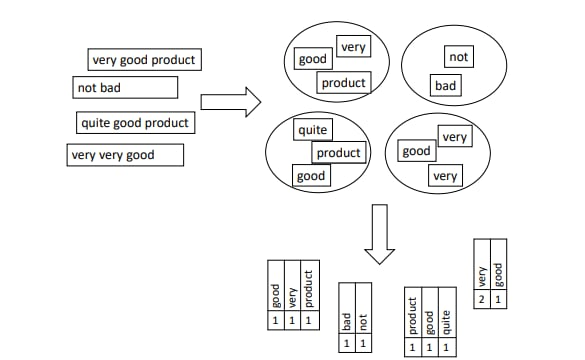
\includegraphics[width = \textwidth]{chapter/chapter3/figure3.2.jpg}
    \caption{The principle of transforming documents (here, examples of very short product
reviews) to bag-of-words.}
    \label{fig:placeholder32}
\end{figure}

\begin{figure}[!ht]
    \centering
    % \includegraphics[width=0.5\linewidth]{}
    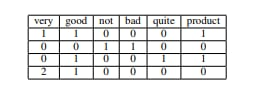
\includegraphics[width = \textwidth]{chapter/chapter3/figure3.3.jpg}
    \caption{A document term matrix created from the documents from Figure 3.2.}
    \label{fig:placeholder33}
\end{figure}

\hspace{-1.5em}must be able to accommodate all possible features and all documents will share
the same features. Of course, some of the documents may not be characterized
by some features (i.e., their value is 0), see Figure 3.2. Now, all documents in a
collection are represented by vectors of the same type and can be arranged into a
table known as the term-document matrix. Such a matrix has a highly structured
format which is suitable for many machine learning algorithms.

\section{The Limitations of the Bag-of-Words Model}

The application of the bag-of-words approach in creating the term-document matrix has a few disadvantages. First, there exist a large number of possible features
which can be derived from texts. When considering words as the most natural
features, even quite a small collection of documents can contain many unique
words. In a data set consisting of 100 hotel accommodation reviews from \textit{booking.com} where the average number of words in a review is about 25, almost 1,000
unique words can be found. In 1,000 documents, we identified more than 3,500
unique words, a collection having 10,000 documents contained almost 13,000
unique words, and in 100,000 documents, about 45,000 distinct words could be
distinguished \cite{ref295}. Such a high number of features is significantly different
from what is typical in classic data mining problems or in relational databases.

The high number of features is often a problem from the computational complexity perspective because processing a larger number of attributes requires
more time. For some algorithms, for example a decision tree induction, the computational complexity grows quadratically with the number of features \cite{ref144}.

Another problem related to the high number of dimensions is known as the
\textit{curse of dimensionality}. Inductive machine learning algorithms try to find a
generalization of the available data. In the case of supervised classification, the goal
is to find a function that is able to assign every item to a correct category (class).
Having a data set with $n$ binary (or boolean) attributes, there exist $2^n$ different
instances. When there are 100 binary attributes, there exist $1.27 \times 10^{30}$ instances.
To learn a perfect function covering the entire instance space, we would need a
huge number of these instances. This is, however, often neither possible nor feasible.
Because of that, we expect that the classifiers will work with some errors and not so
many learning instances are needed. With the use of the PAC-learning
(\textit{probably approximately correct learning}) paradigm, we can even quantify the
relationship between these numbers\cite{ref150}.

The \textit{curse of dimensionality} is a bigger problem for some algorithms than for
others. For example, a $k$-nearest neighbors (k-NN) classifier uses all features to
calculate a similarity between the items in a data set. Thus, the k-NN classifier
is more sensitive to the high number of attributes than, for example, decision
tree or rule learners that work with only a subset of attributes when creating a
generalization of the data \cite{ref199}.

There are two famous statistical laws applicable to natural languages – the
Zipf’s law and Heaps’ law. Zipf’s law says that the frequency of a word (or another
linguistic unit, like a word stem) is inversely proportional to its rank derived
from the frequency of the word in the collection of texts \cite{ref186}. This relationship
can be represented by the following equation:
\[
freq(w_i) = \frac{C}{i^a},
\tag{3.1}
\]

where $freq(w_i)$ is the number of occurrences of the word $w_i$ and $i$ is the position of the word $w_i$
in the list of all words ordered in descending order according
to their frequency (in other words, $i$ is the rank of the word $w_i$). The coefficients
$C$ and $a$ can be derived from the available data having the word counts for every
word appearing in the document collection. Ideally, $C = freq(w_1)$ and $a = 1$. In
that case, the frequency of the second most frequent word will be one half of the
frequency of the most frequent word, the frequency of the third most frequent
word will be one third of the frequency of the most frequent word, etc. The frequency
of the 10th most frequent word will be twice as much as the frequency
of the 20th most frequent word and three times the frequency of the 30th most
frequent word. Zipf’s law was slightly modified by Mandelbrot [184] to better
represent the law, especially for words with high and low ranks:
\[
freq(w_i) = \frac{P}{(i + \rho)^B},
\tag{3.2}
\]

where $freq(w_i)$ is the number of occurrences of the word $w_i$, $i$ is the rank of
the word $w_i$, and the coefficients $P$, $\rho$, and $B$ are derived from the data.
Heaps’ law \cite{ref114} describes the relationship between the size of a data collection
as expressed by the number of words and the number of unique words. This
relationship is demonstrated by the formula:
\[
M = k \cdot N^{b},
\tag{3.3}
\]

where $M$ is the number of unique words, $N$ is the total number of words,
and $k$ and $b$ are coefficients derived from data. Manning, Prabhakar, and Schütze \cite{ref185}
derived the values $k = 44$ and $b = 0.49$ for the Reuters-RCV1 data set.
The typical values of $k$ are between 30 and 100, and $b$ is close to 0.5 (the number of
unique words is thus proportional to the square root of the total number of
words).

The coefficients that appeared in the formulae representing the laws of natural
languages often depend on a specific language; for example, how inflective it is
[98]. However, the laws can give us at least some initial insight to the data and
its statistical characteristics.

For example, when considering the first 10 most frequent words, they should
form about one third of all words in a document collection keeping in mind
the ideal set that conforms to Zipf’s law. Since the data is not ideal, this is not
very exact. However, Manning, Prabhakar and Schutze \cite{ref185} found that the 30 ¨
most common words account for about 30\% of the tokens in Reuters-RCV1. Not
using these words as features in a machine learning task will, on the one hand,
decrease the number of features by a negligible amount. On the other hand, it
will significantly decrease the number of non-zero attribute values. Looking at
the ranked list of words from another perspective, a significant majority of words
appear only a few times. These words are thus often irrelevant for many tasks
(e.g., classification, clustering, or association mining) and can be ignored. They
also often represent some spelling errors so they actually work as a noise. By
removing these words from further processing, a substantial reduction of the
number of features can be achieved.

The large number of features and the implications of Zipf’s law also lead to
an additional problem. When the number of words in the documents is considered, it quite small compared to the number of all unique words in a document
collection. Looking at the previously mentioned collection of customer reviews,
we were able to identify almost 1,000 unique words for the small set consisting
of 100 documents. Taking the average length of 25 words, about 2.5\% of the
vector elements have a non-zero value (when all words in a document are distinct). In the case of the largest collection of 100,000 documents, the percentage
of non-zero items is much smaller, about 0.05\%. We therefore say that the vectors are very sparse which is a problem for some tasks, computing similarity in
classification or clustering \cite{ref177}, for example. The sparsity can also be seen in
the columns of the document-term matrix because a significant number of words
appear only a few times. The sparsity generally means that it is, at times, quite
complicated to identify some patterns in the data \cite{ref87}.

Since word order is not considered, the bag-of-words model has several disadvantages. For example, two sentences with the same words that appear in a
different order will be treated as identical. When word order in a comparative
sentiment analysis task is not taken into consideration, the sentences $A$ is better
than $B$ and $B$ is better than A will look the same although they should lead to
opposite conclusions.

The representations of individual words also bear little semantics. Each word
in the bag-of-words model is just one column in the document-term matrix where
the order of columns is not important. When columns A and B are closer to each other than columns A and C, it does not mean that the words A and B are more
similar in their meaning or grammatical form, for example, than the words A
and C. In the vector space model, all words create one dimension that is equally
important as the others. The distance from the beginning of the vector space of a
position representing, for example, one occurrence of the word A is the same as
the distances of other positions representing one occurrence of any other word.

The issue of the large number of features can be solved by feature selection 
methods (see Chapter~14). The bag-of-words model can also be used
to derive new representations (using, for instance, latent semantic analysis or
neural models creating word embeddings) with fewer dimensions, thus eliminating
the above-mentioned problems. These methods are briefly described in
Chapter~13. The loss of context can be eliminated by working with sequences of
words known as \textit{n-grams} (we therefore sometimes talk about \textit{bag-of-n-grams}) or
by introducing new attributes bearing information about the context of a word
(for example, what is the preceding word, what is the following word, what is
the part-of-speech of the previous word, etc.). Here, however, problems of high
dimensionality and sparseness are often intensified.

Despite the numerous problems and limitations of the bag-of-words model,
it brings surprisingly good results in many tasks. In situations, especially when
there are fewer features, where there is no correlation between them or when we
do not want to take it into account, the bag-of-words approach is appropriate.
Sparse vectors can be also used to learn dense embedding through training a
neural network \cite{ref101}. For example, combining the embedding vectors of words
(through averaging them, for instance) from a document into one vector enables
application of classical machine learning algorithms for classification.

\section{Document Features}

The form taken by the features characterizing documents depends on the problem to be solved. For example, using characters as features might be somehow
useful for a spam filtering task where the presence of some special characters
or too many identical characters can indicate a spam e-mail. On the other hand,
in an information extraction problem where some kind of semantic information
understandable by people is expected as the output, characters as features do not
make much sense. Here, words or concepts play a more important role.

In most cases, the following feature types can be distinguished \cite{ref87}:

\begin{itemize}
    \item \textit{Characters, character bi-grams, tri-grams, n-grams:} In spite of being
the most complete representation of textual data, characters are not often
used as features. The reason is quite simple – one character does not bear
much semantic information, so any interpretation is quite complicated,
especially when the positional information, i.e., information about the context
of a character, is lost (we can thus talk about a \textit{bag-of-characters}
representation).

    \item \textit{Words:} Words are the most natural and straightforward features that can
be derived from texts. A word is a sequence of symbols, typically letters, that is
used in the sentences of a given language. It has a semantic, grammatical, and
phonological unity and is usually separated from other words by spaces in writing \cite{ref74}.
This is how words are understood by most Western languages. On the other hand,
texts in, for instance, Chinese or Arabic do not usually contain spaces between words,
so it is not easy to visually identify their borders.

A dictionary can be used to find out what is and what is not a word in
a given text. It is quite typical that a dictionary — a list of words that are
available in the given language — exists for a natural language. The
dictionaries might contain only the basic form of the given word, called
\textit{lemma}. For example, the lemma for \textit{does}, \textit{doing}, \textit{done}, or \textit{did} is
\textit{do}. Therefore, the absence of a particular sequence of characters in a
dictionary does not necessarily mean that it is not a proper word.

What about other parts of texts, like numbers, temporal expressions, currency symbols, and punctuation (comma, period, question mark, quotation marks, etc.)? It generally depends on the task to be performed. Sometimes, a particular number or date can be important. If the number is, for
example, the price of a product, we can use a specific value to find out
whether the product is expensive or cheap. Sometimes it is enough to
know that the text shows specific price.

One of the disadvantages of using words is that, without a context, the
possible meaning of a word may not be obvious.

    \item \textit{Terms:} Terms are single words or multiword expressions formed of words
from the text. When looking at the fictive news headlines mentioned earlier in this
chapter, terms like \textit{Las Vegas}, \textit{ice hockey}, \textit{FIFA World Cup}, or
\textit{the National Lottery} can be identified. Since more words are treated as
one unit, the ambiguity of words is reduced.

    \item Term extraction is related to the Named Entity Recognition (NER) problem, 
which is a subtask of Information Extraction. Its goal is to identify information 
units like names (typically persons, organizations, and locations) and numeric 
expressions including time, date, money, and percent expressions \cite{ref205}.

    \item \textit{Concepts:} Concepts are features that are generated from the text based
on the occurrence of words, phrases, or more complicated structures. The
concepts do not have to appear directly in the text. In the case of news
headlines, for example, concepts like \textit{sport} or \textit{gambling} can be identified.

Concepts, together with terms, have the most expressive semantic value.
Concepts enable better handling of synonymy, polysemy, hyponyms, or
hypernyms. On the other hand, they require more effort to be extracted.
They are also often domain dependent.

Assigning correct concepts often involves cross-referencing against a
source of external knowledge which can be the knowledge of a domain
expert, an existing ontology or lexicon, or an annotated collection of
training documents used to train an algorithm assigning concepts.
\end{itemize}

Characters or words can be combined to form character or word n-grams.
A character n-gram is a sequence of n consecutive characters. A few character
3-grams created from this sentence include “A f”, “ fe”, “few”, “ew ”, “w 3”,
etc. Word 2-grams from this sentence include “Word 2-grams”, “2-grams from”,
“from this”, etc.

The character n-grams are able to capture whole words (“few”) as well as
word class (e.g., “ed ”, “ing”). A great advantage of character n-grams when
compared to word n-grams is that they do not create as many dimensions (the
sparsity of data is lower) because there exist fewer character combinations
than word combinations \cite{ref139}. Character n-grams have been successfully used
for many tasks, including language identification \cite{ref38}, authorship identification
\cite{ref118}, malicious code detection \cite{ref223}, and plagiarism detection \cite{ref17}.

Word n-grams can help in capturing multiword phrases \cite{ref163} and have been
successfully used in sentiment analysis \cite{ref273}.

An interesting collection of word n-grams, together with their frequency of
usage in books, is provided by Google. Their new edition of the \textit{Google Books
Ngram Corpus} provides syntactically annotated n-grams for eight languages and
covers about 8\% of books that have been ever published (more than 8 million
books) \cite{ref172}.

N-grams can be also understood as a simple statistical language model that
models probabilities of sequences of characters or words. In other words, given
a sequence of previous words, the model can help us predict a word. As such, it
can be successfully used in task, such as machine translation, spelling correction,
or speech recognition \cite{ref138}.

\section{Standardization}

Text data is commonly presented in some kind of semi-structured representation.
A web page containing the most recent news might include several news features
consisting of a heading, list of keywords, a few paragraphs of text, images with
captions, etc., all enclosed within \texttt{<div>} or similar tags with defined classes.

For example, an XML file containing news from Reuters Corpus Volume 1
(RCV1) \cite{ref167} consists of elements containing the publication date, related topic, mentioned people, places or organizations and the text consisting of a title, date
line, and body (see Figure 3.4).

\begin{verbatim}
<?xml version="1.0" encoding="iso-8859-1" ?>
<newsitem itemid="2286" id="root" date="1996-08-20" xml:lang="en">
  <title>MEXICO: Recovery excitement brings Mexican markets
  to life.</title>
  <headline>Recovery excitement brings Mexican markets
  to life.</headline>
  <byline>Henry Tricks</byline>
  <dateline>MEXICO CITY</dateline>
  <text>
    <p>Emerging evidence that Mexico’s economy was back on the
    recovery track sent Mexican markets into a buzz of excitement
    Tuesday, with stocks closing at record highs and interest
    rates at 19-month lows.</p>
    <p>&quot;Mexico has been trying to stage
    ...
    </p>
  </text>
  <copyright>(c) Reuters Limited 1996</copyright>
  <metadata>
    <codes class="bip:countries:1.0">
      <code code="MEX">
        <editdetail attribution="Reuters BIP Coding Group"
        action="confirmed" date="1996-08-20"/>
      </code>
    </codes>
    <codes class="bip:topics:1.0">
      <code code="E11">
        <editdetail attribution="Reuters BIP Coding Group"
        action="confirmed" date="1996-08-20"/>
      </code>
      ...
    </codes>
    <dc element="dc.publisher" value="Reuters Holdings Plc"/>
    <dc element="dc.date.published" value="1996-08-20"/>
    ...
  </metadata>
</newsitem>
\end{verbatim}

\begin{figure}[H]
    \centering
    \caption{An example of an XML file containing a newspaper article from the RCV1 document collection.}
    \label{fig:placeholder34}
\end{figure}

A JSON (JavaScript Object Notation) file stores the data in a human readable
format as objects consisting of name/value pairs where the value can be a scalar
(string, number, logical value), another object, or a list of values \cite{ref79}.

With a semi-structured document, only the content of some selected elements
might be important for a specific task. For example, to train a classifier to categorize
newspaper articles, only the content of elements \texttt{<code>} in the 
\texttt{<codes class="bip:topics:1.0">} section, \texttt{<title>}, and \texttt{<text>} is relevant. 
The content of \texttt{<title>} and \texttt{<text>} will be the base for deriving 
document features, while the content of \texttt{<code>} element will be used to specify 
the class labels (one or more) for the documents.

The XML library can be used to process XML (and HTML) documents. The
\texttt{xmlToList()} function converts an XML document or node to a list that directly
contains the data. The list elements correspond to the children of the top-level
node, and the \texttt{.attrs} element is a character vector of attributes from the node.

\begin{verbatim}
> library("XML")
> data<-xmlToList("Reuters/CD1/2286newsML.xml")
> names(data)
[1] "title" "headline" "byline" "dateline" "text"
[6] "copyright" "metadata" ".attrs"
> data["title"]
$title
[1] "MEXICO: Recovery excitement brings Mexican
markets to life."
> data$metadata$codes$code$.attrs
code
"MEX"

\end{verbatim}

The following example (from [143]) shows how to extract information about
reviews of conference papers. The file with the information in the JSON format
contains one object with key papers. The value associated to this key is an array
where every element represents one paper. Every paper has a numeric identifier,
a string value representing a preliminary decision on the paper, and the list of
reviews. The reviews contain information about reviewers’ confidence, evaluation of the paper on a given numeric scale, the number of the review, language,
text of the review, additional remarks to the conference committee, date of the
reviews, and authors’ evaluation of the review. An excerpt from the JSON file
can be found in Figure 3.5.

The \texttt{fromJSON()} function from the rjson package converts a string containing a JSON object, the content of a file, or the content of a document with a
given URL to an R object. The type of the object is list. Its elements are num-

\begin{verbatim}
{
  "paper": [
    ...
    {
      "id": 8,
      "preliminary_decision": "accept",
      "review": [
        {
          "confidence": "4",
          "evaluation": "1",
          "id": 1,
          "lan": "en",
          "orientation": "0",
          "remarks": "",
          "text": "The paper describes an experience concerning...",
          "timespan": "2010-07-05"
        },
        {
          "confidence": "4",
          "evaluation": "2",
          "id": 2,
          "lan": "en",
          "orientation": "1",
          "remarks": "",
          "text": "This manuscript addresses an interesting solution...",
          "timespan": "2010-07-05"
        }
    },
    {
      "id": 12,
      "preliminary_decision": "accept",
      "review": [
        {
          "confidence": "4",
          "evaluation": "2",
          "id": 1,
          "lan": "es",
          "orientation": "2",
          "remarks": "Se trata de un articulo que presenta un tema ...",
          "text": "Es un articulo que presenta un tema novedoso ...",
          "timespan": "2010-07-05"
        },
        ...
    },
    ...
  ]
}
\end{verbatim}

\begin{figure}[H]
    \centering
    \caption{An example of a JSON file containing information about reviews of papers from
a conference.}
    \label{fig:placeholder35}
\end{figure}

\hspace{-1.5em}bered when they come from a list of values in a JSON object and have names
when they are converted from an object with name/value pairs.

\begin{verbatim}
> library("rjson")
> data <- fromJSON(file="reviews.json")
> names(data)
[1] "paper"
> names(data[[’paper’]][[1]])
[1] "id" "preliminary_decision"
[3] "review"
> names(data[[’paper’]][[1]][["review" ]][[1]])
[1] "confidence" "evaluation" "id" "lan"
[5] "orientation" "remarks" "text" "timespan"
> # a piece of text of the first review of the first paper
> substr(data[["paper"]][[1]][["review"]][[1]][["text"]],
+ 1, 60)
[1] "- El articulo aborda un problema contingente y muy
relevante"
> # the language of the first review of the first paper
> data[["paper"]][[1]][["review"]][[1]][["lan"]]
[1] "es"
> # a decision on the first paper
> # same as data[[1]][[1]][[2]]
> data[["paper"]][[1]][["preliminary_decision"]]
[1] "accept"
\end{verbatim}

The following commands convert the data to a data frame with two columns,
Text and Evaluation. The data can be used, for example, in a classification
task where the evaluation will be predicted according to the text of reviews.

\begin{verbatim}
# creating an empty data frame
d <- data.frame("Text"=c(),
                "Evaluation"=c(),
                stringsAsFactors=FALSE)
for (i in 1:length(data[["paper"]])) {
 # looking at the number of reviews of the ith paper
nr <- length(data[["paper"]][[i]][["review"]])
if (nr==0) {next}
for (r in 1:nr) {
 # adding the text and evaluation to the data frame d
 d <- rbind(d,
            data.frame(
            "Text"=data[["paper"]][[i]][["review"]]
                        [[r]][["text"]],
            "Evaluation"=data[["paper"]][[i]]
                             [["review"]][[r]]
                             [["evaluation"]]
           )
          )
   }
}

\end{verbatim}  

\section{Texts in Different Encodings}

Texts are stored in computer memory as a sequence of bits. Each character then
usually occupies a certain number of bytes. To order to be stored, a character
needs to be encoded to a number. It needs to be decoded to display a character.

In the past, seven bits enabling the storage of 128 distinct characters were
needed to encode a character. This was enough for English letters, digits, and
some other common symbols like punctuation.

However, for some other languages, like German, Spanish, French, Czech,
etc., characters with accents were needed. It was not possible to encode all these
characters to a 7-bit character, so eight bits were used. Different languages had
different encodings. For some languages, like Chinese, even eight bits were not
enough \cite{ref210}. This problem can be solved using the Unicode encoding, which is
a de facto standard in simultaeously encoding many languages and scripts \cite{ref109}.

Knowledge of text encoding is necessary for some of the preprocessing steps,
like tokenization, for example. In some languages, characters encoded by some
numbers are regular word characters while in others they are punctuation characters \cite{ref210}.

Document encoding can be explicitly indicated as, for example, in some
metadata or headers of a document. In certain contexts, an explicit or implicit
agreement on a specific encoding might be made as well. When no such information is available, a user or computer must make a guess based on an inspection
of the text \cite{ref149}.

To guess a document encoding in R, the stri enc \texttt{detect()} function from
package indexR packages\texttt{!stringistringi} can be used. The function accepts a
character vector and returns a list of guessed encodings, language, and confidence level for each string. It currently supports about thirty different character
sets and languages.

\begin{verbatim}
texts <- c(
  "What is your name?",
  "¿C´omo te llamas?",
  "Comment tu t’apelles?"
)
stri_enc_detect(texts)

[[1]]
Encoding     Language  Confidence
1 ISO-8859-1  en        0.47
2 ISO-8859-2  hu        0.31
3 UTF-8       0.15
...

[[2]]
Encoding     Language  Confidence
1 UTF-8       0.80
2 ISO-8859-1  es        0.47
3 ISO-8859-2  hu        0.15
...

[[3]]
Encoding     Language  Confidence
1 ISO-8859-1  fr        0.71
2 UTF-8       0.15
3 ISO-8859-2  hu        0.14
\end{verbatim}

Texts can be converted from one encoding to another using the standard \texttt{iconv()} function. The list of available encodings is provided by the
\texttt{iconvlist()} function.

\begin{verbatim}
> x<- "Gr\xfc\xdf Gott"
> x
[1] "Gr¨uß Gott"
> Encoding(x)
[1] "unknown"
> Encoding(x) <- "latin1"
> Encoding(x)
[1] "latin1"
> xx <- iconv(x, from="latin1", to="UTF-8")
> Encoding(xx)
[1] "UTF-8"
\end{verbatim}

\section{Language Identification}

Some of the preprocessing steps, like tokenization, stemming, or part of speech
tagging are language dependent. Language identification is actually a categorization problem – a language label is assigned to a text.

A straightforward approach can compare words of a text with dictionaries of
known languages and assign the language with the highest match as the correct
one. Typically, texts are compared with only the most frequent words in a language. The accuracy of these methods is, however, not very high, especially for
short texts \cite{ref106}.

Other approaches work with variable or fixed length character n-grams. The
n-grams in a text are compared to an n-grams based model of a language. The
model can be based on simple frequencies of n-gram occurrences \cite{ref44} or can
have the form of a probabilistic Markov model \cite{ref215}.

A comparison of some popular language identification algorithms can be
found in \cite{ref131}.

To determine a language, for example, R provides, the \texttt{cld2} (Google’s Compact Language Detector 2) package and its function \texttt{detect language()}.

\begin{verbatim}
texts <- c("What is your name?",
           "¿C´omo te llamas?",
           "Comment tu t’apelles?",
           "Wie heißt du?",
           "Jak´e je tvoje jm´eno?")
detect_language(texts)
[1] "en" "es" "fr" "de" "cs"
\end{verbatim}  

\section{Tokenization}

Tokenization is the process of splitting a document into pieces of texts known as
\textit{tokens}. These tokens are often the words contained in the text. In most European
languages where the words are space delimited, the task seems to be quite simple
– to split the text at the places where are white spaces. In some other languages,
like Chinese, where there are no spaces between words, the text needs to be
analyzed in greater depth.

Even in European languages, the process is usually not that straightforward.
Punctuation (including brackets, apostrophes, dashes, quotation marks, period,
exclamation mark) is usually understood as something separating the tokens. Besides removing white spaces, punctuation marks are usually removed too which
is probably the simplest tokenization approach \cite{ref275, ref211}.

There are, however, many exceptions and special problems related to different languages. Even for English, tokenization is not an easy task. The following
text mentions a few typical problems.

A period is usually understood as the end of a sentence. It can be, however,
used for other purposes, like in abbreviations (\textit{Mr., etc., U.S.A.}) or in numbers in
English (1.23). In such cases, the period is often a part of the tokens.

Apostrophes can be used in contractions (\textit{I’m}, \textit{haven’t}), genitive forms of
nouns (\textit{Peter’s}), or when omitting the first two digits in a year (\textit{’90s}). We then
need to decide whether the apostrophe should be removed (\textit{haven’t} $\to$ \textit{haven + t}),
retained, or replaced (\textit{’90s} $\to$ \textit{1990s}). In many situations, it is still not clear
what should happen. For example, should \textit{doesn’t} be transformed to \textit{doesnt}, 
\textit{doesn+t}, or \textit{does+n’t}?

Several words can also be connected by hyphens to create compound words
(\textit{state-of-the-art}, \textit{bag-of-words}, \textit{two-year-old}, 
\textit{sugar-free}, \textit{long-lasting}). Should
we treat each part of the compound expression separately or the whole expression
as one token?

Special attention should be given to numbers. Numbers can be written in
many different ways, including a decimal point (comma in some languages),
$+$ or $-$ sign, semilogarithmic notation, etc. When a phone number is treated
as one token, we cannot see, for example, an area code (\textit{00420-777777777} vs.
\textit{00420+777777777}). The same might be applied to dates: \textit{2018-02-14} can be
treated as one token as well as \textit{2018+02+14}, so we have information about the year,
month, and day.

Other pieces of text that require special attention are, for example, e-mail
addresses, URLs, special names (\textit{C++, Bell\&Ross}) among others.

Some languages, like German, often use compound words that are not hyphenated. For example, the longest German word in 2013 \cite{ref265}\textit{Rindfleischetikettierungsuberwachungsaufgabenubertragungsgesetz} refering to the law for the
delegation of monitoring beef labelling consists of ten words. Some of them are
prefixes, but can also be prepositions and are counted as words here. Thus, the
long word consists of ten words.

It is obvious that tokenization is a language specific task. The language of a
text must therefore be known for tokenization that is not naive. The rules defining some specific tokens in a language must be clearly stated. The process of
tokenization is also influenced by the used text encoding because delimiters and
special symbols occupy different positions in different character tables \cite{ref211}.

\section{Sentence Detection}

In some tasks, splitting a document into smaller units, like sentences, can be
beneficial. It seems that finding symbols which normally end sentences, like .,
\texttt{?}, or \texttt{!} should be enough. These symbols can, however, also be parts of other expressions (for example, a period can be a part of an abbreviation or a number).
A terminating symbol can be also omitted, like in the case when a sentence ends
with an abbreviation.

A human expert can define a set of rules to be used to separate sentences
(e.g., the symbol, like a period, must be followed by a whitespace and an uppercase letter). As manual creation of such rules need not be the best approach, an
algorithm can be trained to detect sentences from labeled data \cite{ref225}.

In R, sentences can be extracted from a text using the \texttt{udpipe()} function
from package udpipe. For more details, see the example at the end of this chapter.

\begin{verbatim}
> unique(udpipe("I’m Mr. Brown. I live in the U.S.A.",
+               object="english"
+              )[’sentence’]
+       )
               sentence
1       I’m Mr. Brown.
6 I live in the U.S.A.
\end{verbatim}  

\section{Filtering Stop Words, Common, and Rare Terms}

Some of the words that are too common do not usually contribute (or contribute
only negligibly) to achieving a certain goal. For example, in the query \textit{Find a
hotel in Prague} submitted to a web search engine, the word a does not influence
what will be retrieved by the search engine. The retrieved results will be the same
no matter whether a is or is not in the query. The reason is simple – almost all
documents written in English contain at least one occurrence of the word a. On
the other hand, the word \textit{Prague} is very important because without it the search
engine would return information about hotels in many other locations.

Similar importance of words is apparent in other text mining tasks, such as
classification or clustering. When categorizing, for example, newspaper articles
to categories, the occurrence of word the will not play an important role because
articles from all categories are very likely to contain this word. In a clustering
process, when calculating the similarity between two documents, the occurrence
of the word the will contribute to the similarity measure with the same value for
almost all document pairs.

It is obvious that the words not contributing to achieving a certain goal are
useless and do not have to be considered in further processing.

The words that are not important for a certain task are known as \textit{stop words}.
Very often, they are the most frequent words in a given language. Typical stop
lists for English contain words like \textit{the}, \textit{of}, \textit{and}, \textit{by}, 
\textit{with} (grammatical articles, prepositions, conjunctions, auxiliary verbs, pronouns, articles). 
Many stop word lists can be found on the web or incorporated in various tools and in the libraries
of programming languages. Table~3.1 shows how the numbers of stop words
for different languages can differ (the table is based on stop lists in Python’s
NLTK library v.~3.4). It is, however, obvious that the number of stop words is
usually around a few hundred. It should be noted that the available stop word lists
sometimes suffer from surprising omissions and inclusions, or are incompatible
with particular tokenizers\cite{ref207}. Various stop word lists in R can be obtained
from the function \texttt{stopwords()} from the \texttt{tm} package.

The stop word list length, when compared to the size of the dictionary, which
can be a few hundreds of thousands, is negligible. The number of features thus
does not decrease significantly when stop words are removed. A massive reduction is, however, noticeable in the total number of words (which is related, for
example, to the memory requirements). According to Zipf’s law, ten most frequent words represent approximately one third of all words in a corpus.

A stop list can also be easily created by simply counting the frequencies of
words in a corpus and looking at the most frequent words. It is, however, better
to carefully examine the frequent words so that important words are not lost.

What is and what is not a stop word might depend on a domain. In a collection
of hotel accommodation reviews, the word hotel would probably be very frequent
and will not be useful in, for example, determining whether a review is negative,
positive, or neutral. In the following example, reviews from booking.com (for
a detailed description of the data, see \cite{ref295}) are processed. The number of all
words, unique words, and global words frequencies are calculated from a matrix
representing the documents. The frequencies together, with relative frequencies
of the ten most frequent words are printed. Subsequently, the 50 most frequent
words are displayed without their frequencies. We can see that the list contains
typical English stop words as well words typical for the hotel accommodation
domain. From a sorted list of words together with their frequencies, a graph
demonstrating Zipf’s law can be easily generated (with logarithmic axes).


\begin{table}[H]
\centering
\caption{Numbers of stop words for different languages in stop lists in Python’s NLTK library v.~3.4.} 
\vspace{2em}
\begin{tabular}{l|c}
\hline
\textit{Language} & \textit{Number of Stop Words} \\
\hline
English & 179 \\
German & 231 \\
Italian & 279 \\
French & 155 \\
Spanish & 313 \\
Russian & 151 \\
\hline
\end{tabular}
\end{table}

\begin{verbatim}
> library(tm)
> text <- readLines("reviews-booking.txt")
> corpus <- VCorpus(VectorSource(text))
> corpus <- tm_map(corpus, removePunctuation)
> corpus <- tm_map(corpus, stripWhitespace)
> corpus <- tm_map(corpus, content_transformer(tolower))
> dtm <- DocumentTermMatrix(corpus)
> mat <- as.matrix(dtm)
> word_frequency <- colSums(mat)
> number_of_words <- sum(word_frequency)
> unique_words <- length(word_frequency)
> paste("The number of all words: ", number_of_words)
[1] "The number of all words: 394993"
> paste("The number of unique words: ", unique_words)
[1] "The number of unique words: 19528"
# printing a word together with its rank, total frequency,
# and relative frequency
> words_sorted <- sort(word_frequency, decreasing = TRUE)
> for (i in 1 : 10) {
+   print(paste("word: ", i, ": ",
+               names(words_sorted[i]),
+               ", freq.: ", words_sorted[i],
+               ", rel. freq.: ",
+               round((words_sorted[i]/number_of_words),3),
+               sep=""
+              )
+         )
+  }
[1] "word 1: the, freq.: 33313, rel. freq.: 0.084"
[1] "word 2: and, freq.: 18681, rel. freq.: 0.047"
[1] "word 3: was, freq.: 13445, rel. freq.: 0.034"
[1] "word 4: very, freq.: 8644, rel. freq.: 0.022"
[1] "word 5: room, freq.: 6969, rel. freq.: 0.018"
[1] "word 6: hotel, freq.: 6742, rel. freq.: 0.017"
[1] "word 7: for, freq.: 6092, rel. freq.: 0.015"
[1] "word 8: staff, freq.: 5447, rel. freq.: 0.014"
[1] "word 9: good, freq.: 4819, rel. freq.: 0.012"
[1] "word 10: not, freq.: 4361, rel. freq.: 0.011"

# Printing 50 most frequent words
> names(words_sorted[1:50])
 [1] "the"        "and"        "was"        "very"
 [5] "room"       "hotel"      "for"        "staff"
 [9] "good"       "not"        "were"       "location"
[13] "breakfast"  "with"       "but"        "clean"
[17] "friendly"   "from"       "nice"       "had"
[21] "there"      "helpful"    "rooms"      "that"
[25] "have"       "excellent"  "you"        "this"
[29] "great"      "our"        "are"        "all"
[33] "comfortable" "stay"      "would"      "they"
[37] "small"      "close"      "only"       "one"
[41] "well"       "could"      "which"      "food"
[45] "service"    "city"       "also"       "night"
[49] "bathroom"   "when"

# plotting the curve demonstrating the Zipf’s law
> plot(words_sorted, type="l", log="xy",
+      xlab="Rank", ylab="Frequency")
\end{verbatim}

Special attention should be paid to \textit{stop words} in \textit{multiword expressions} and
to words that are somehow affected by the occurrence of a stop word. Consider
the following phrases: \textit{room with balcony} and \textit{room without balcony}, or \textit{good} and
\textit{not good}. Leaving the stop words (\textit{with}, \textit{without}, \textit{not}) out of consideration, the
meaning of the phrase will change significantly (in fact, it will be the opposite).
There are also phrases consisting solely of stop words, like \textit{The One} (a movie),
\textit{to be or not to be} (a famous phrase from Shakespeare’s \textit{Hamlet}), or \textit{The Who}
(an English rock band). Weiss \textit{et al.} \cite{ref275} thus recommend the removal of stop
words after the features for a document set are created and other preprocessing
techniques (e.g., \textit{stemming}) have been applied.

While \textit{stop words} appear at the top of a list of words ordered by their frequency, 
the words at the other end of the list can also be eliminated. Consider a 
\textit{classification problem} where there are 1,000 documents in two classes, 
$C_1$ and $C_2$. Only one document, $d$, from the entire collection contains 
one specific word $w$. The document belongs to class $A$. The word $w$ is 
definitely helpful and can be used when assigning documents to $A$. 
The rule ``if a document contains $w$ it should be assigned to $A$'' will cover 
${1}/{1000}$ of the training examples and is therefore not too general. 
Having too many such rules will very likely lead to \textit{overfitting} of a classifier, 
which is not desirable. Not considering $w$ by a classifier can cause 
${1}/{1000} = 0.1\%$ error on the training data, which is also negligible.

In the calculation of the similarity of two documents during clustering, the
words with low frequencies will not have an effect on the results because there

\begin{figure}[!ht]
    \centering
    % \includegraphics[width=0.5\linewidth]{}
    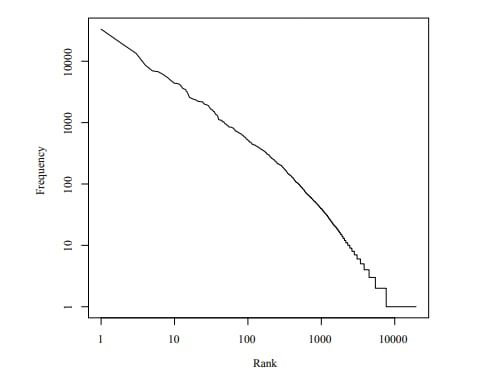
\includegraphics[width = \textwidth]{chapter/chapter3/figure3.6.jpg}
    \caption{Graphical demonstration of Zipf’s law.}
    \label{fig:placeholder36}
\end{figure}
\hspace{-1.5em}is actually no similarity in the given dimension when one document contains a
word and the other does not.

It seems that removing rare words is a good idea for most of the tasks. Sometimes, the computational complexity of a problem can be lowered significantly,
especially for algorithms, where the complexity grows exponentially with the
number of features. On the other hand, in an information retrieval task, not considering those rare words (for example, a specific name of a person, place, or
company) can result in the failure to achieve a certain goal. Here, the document
containing one specific word will not be found by a search engine. Indexing rare
terms thus increases the success rate of a search engine but, on the other hand,
might decrease its performance because more terms would need to be stored and
processed.

\section{Removing Diacritics}

Diacritics (diacritical marks, accents) are symbols added to letters, usually above
or below. Diacritics often changes the way a sound is pronounced (e.g., longer,
with an accent). In some languages, like in Vietnamese, Czech, Spanish, or
French, diacritics are quite common. In some situations, they help distinguish between two completely different words like in Spanish – como ´ (how) and como
(I eat), or French – \textit{cote} (quota), \textit{cote´} (respected), \textit{cote ˆ} (coast), or \textit{cotˆ e} (side).
The removal of accents can thus, sometimes lead to the loss of very important
information.

It is, therefore, necessary to look at the data and think about the process of its
creation. In the past, many SMSs and e-mails were written without diacritics, so
some normalization could be useful.

In English, almost no accents are used and their potential removal does not
usually cause major problems (e.g., \textit{na\"{\i}ve} $\rightarrow$ \textit{naive}).

In R, most versions of the \texttt{iconv()} function enable diacritics removal by
appending \texttt{//TRANSLIT} to the output encoding.

\begin{verbatim}
> x <- "Dobr´y den, ˇclovˇeˇce!"
> iconv(x, from="CP1250", to="ASCII//TRANSLIT")
[1] "Dobry den, clovece!"
\end{verbatim}

\section{Normalization}

The goal of normalization is to convert tokens that look differently (are, for example, written in a different letter case) but have the same meaning to the same
form [263].

\subsection{Case Folding}

Case folding is the process of converting all characters of a word to the lower
or upper case (the lower case is more common \cite{ref62}). When two or more words
with the same meaning are written with different casing, the number of unique
words increases unnecessarily and it is, therefore, favourable to convert them
to one form. The reasons why the same word is written with different casing
might include the position at the beginning of a sentence, presence in a title, the
intention to emphasize a word, etc.

Some words, on the other hand, require capitalization and folding the case
in these situations changes the meaning of the word. Typically, names of people,
places, companies, etc. are written with the first letter capitalized. For example,
\textit{bush} in the middle of a sentence means a small, woody plant, while 
\textit{Bush} would probably mean the former American president (when 
\textit{Bush} is at the beginning of a sentence, it could be either). After conversion 
to lower case and not being aware of the context, one cannot distinguish whether 
a text is about plants or politics according to the occurrence of the word 
\textit{bush}. Abbreviations, although sometimes looking like regular words, are 
written in the upper case. \textit{SMART} (System for the Mechanical Analysis and 
Retrieval of Text) when converted to lower case is a synonym for \textit{intelligent}.

Case folding can be problematic in some specific languages. For example, in
French, accents are optional for uppercase. The word \textit{P\`ECHE} can be converted
to \textit{p\`eche}, which means \textit{fishing}, \textit{peach}, or \textit{p\'ech\'e} meaning \textit{sin}.

Capitalization plays an important role in some languages \cite{ref102}. For example,
all nouns are capitalized in German. For instance, Recht as a noun means law
while recht as an adjective means right. The letter ß also exists only in lower
case.

Intelligent case folding is a machine learning problem. As an alternative, a
simple approach can convert all words at the beginning of sentences as well as
the words from titles and headings to lower case. The case of other words can be
retained \cite{ref6}.

\subsection{Stemming and Lemmatization}

A \textit{word} is the smallest lexical unit of a language that can be used in isolation.
A \textit{morpheme} is the smallest unit of a word that carries some semantic or grammatical meaning. Morphemes typically include prefixes, suffixes, and a root. For
example, the word \textit{unexpected} consists of three morphemes -- a prefix \textit{un}, 
a root \textit{expect}, and a suffix \textit{ed}. Some morphemes can be used in a language 
by themselves (\textit{expect}) while not the others (\textit{un}, \textit{ed}). The former are 
known as \textit{free forms}, the latter as \textit{bound forms}\cite{ref11}.

Stems are parts of words that carry the basic meaning. When a stem consists
of a single morpheme, it is identical to the root. Free stems can occur alone
whereas bound stems cannot.

Words are formed in a \textit{word-formation process} using several rules. 
For example, a plural morpheme \textit{s} can be added to a singular noun to create a plural noun 
(e.g., \textit{book} $\rightarrow$ \textit{books}). One major morphological operation is the use of 
\textit{inflection}, which is the addition of a plural, possessive, plural+possessive, comparative, 
superlative, 3rd person singular, past tense, past participle, or present participle forms to a stem. 
The second type of word-formation operation is \textit{derivation}, which includes adding 
adjective derivational affixes (\textit{day} $\rightarrow$ \textit{daily}, \textit{depend} $\rightarrow$ 
\textit{dependent}, \textit{help} $\rightarrow$ \textit{helpful}, etc.), adverb derivational affixes 
(\textit{slow} $\rightarrow$ \textit{slowly}, or \textit{clock} $\rightarrow$ \textit{clockwise}), 
and many others~\cite{ref126}. Inflection never changes the category of a word 
(e.g., a noun will still be a noun after adding a suffix), while derivation 
can change the category (a noun can become an adjective after adding a suffix).

It is obvious that the \textit{semantic meaning} of some words, when created from
the same stem, is very close. When a newspaper article contains one of the words
\textit{sport}, \textit{sports}, \textit{sporting}, \textit{sported}, or \textit{sporty}, it is quite likely 
to be an article from the \textit{sports category}. However, for a computer, all five words are 
different, and to assign an article correctly to the category, all five words need to be 
connected to it, for example, in a \textit{classification rule}.

The goal of the procedure known as \textit{stemming} is to convert all different forms
of a word to one common form known as the \textit{stem}.

To find a correct \textit{stem}, a \textit{morphological analysis} of the word is often necessary. 
However, many \textit{stemmers} (a stemmer is a function or a program performing 
stemming) employ simple rules to strip affixes. This can lead to a situation where 
the difference between, for example, a noun and a verb disappears -- a noun 
\textit{driver} and a verb \textit{driving} will be stemmed to \textit{driv}. We can also see that 
\textit{driv} is not a correct dictionary word. Some of the stemmers are not constrained 
to produce only real words~\cite{ref189}. This is usually not considered a deficiency 
because the word is often used as a feature in a \textit{machine learning task} and not 
as a piece of a message for a human. At the same time, when a stem changes with 
the addition of a suffix (e.g., \textit{index}~$\rightarrow$~\textit{indices}), a simple stemmer will not 
convert different variants to a common one.

It is obvious that a \textit{stemming process} is not error-free. The errors include 
\textit{understemming} (the found stem does not cover all word variants) and 
\textit{overstemming} (a word is shortened too much so it covers words with different meanings). 
Understemming is usually achieved by \textit{light stemmers} that prefer precision 
over recall, while \textit{aggressive stemmers} preferring recall often overstem 
the words~\cite{ref39}.

The most famous \textit{stemming algorithm} for English text, belonging to the 
group of \textit{rule-based stemmers}, is \textit{Porter’s algorithm}~\cite{ref217}. It uses five groups of 
rules that are successively applied to strings, for example, 
\texttt{SSES~$\rightarrow$~SS} (\textit{caresses~$\rightarrow$~caress}), 
\texttt{ATIONAL~$\rightarrow$~ATE} (\textit{relational~$\rightarrow$~relate}), 
\texttt{ALIZE~$\rightarrow$~AL} (\textit{formalize~$\rightarrow$~formal}), or 
\texttt{AL~$\rightarrow$~""} (\textit{revival~$\rightarrow$~reviv}). 
The rules can contain conditions, such as whether the stem contains a vowel, 
ends with a double consonant, or is longer than a given length, etc.

Porter \cite{ref218} also developed a system for defining stemming algorithms. The
rules of stemming algorithms are expressed in a natural way in a simple language
known as Snowball. A Snowball compiler then translates a Snowball definition
into an equivalent program in ANSI C or Java.

Dictionary stemmers need a dictionary containing all variants (inflected
forms) of a word together with their stems. This method is not suitable for languages with many words and for heavily inflected languages \cite{ref140}.

Rule based and dictionary stemmers require that the rules be constructed by
linguistic experts for a specific language. As they are not able to handle situations
which are not covered by the rules or the dictionary, statistical or machine learning approaches would be better in some situations. For example, the algorithm
of Bacchcin, Ferro, and Melucci et al. \cite{ref15} estimates the most probable split into
the stem and suffix from all possible splits for each word in the full corpus. In
\cite{ref39}, the authors clustered together words occurring in similar contexts and sharing a common prefix of at least a minimum length. Such words are expected to
be semantically and lexically similar; this can be enough to replace them by one form. They are, however, taken as the training data for a classifier which learns
stemming rules so that processing unseen data is possible.

Lemmatization converts a word to its dictionary form known as the lemma.
To be able to perform such a conversion, deeper knowledge than that required
for stemming is needed. A lemmatizer usually needs a complete vocabulary and
morphological analysis to correctly lemmatize words \cite{ref185}. The words like better or thoughts can be converted to their correct forms good and think, which
would not be achieved by a stemmer. Attempts to train a lemmatizer, like in
\cite{ref14,ref136}, have also been made but they are not error free.

\subsection{Spelling Correction}

Mistypings are common problems in any written text. The problem is that they
bring noise to the data which can complicate the achievement of satisfactory
results in some tasks. \textit{Spelling correction} is a solution to this problem. Generally,
the process of spelling correction involves detection of an error, generation of
candidate corrections, and ranking of candidate corrections \cite{ref155}.

Mistypings can be detected by comparing each word to an existing dictionary
or looking at every character n-gram (n is usually 1, 2, or 3) to determine whether
such an n-gram exists for a given language.

When an error is found, our response is to correct it. The correction can be
done with or without taking into consideration, the context of the error. The methods which do not take the context into consideration suppose that most of the errors are caused by insertion, deletion, substitution, and transposition; they appear
in the middle of a word, can be related to a computer keyboard arrangement, etc.

Sometimes, knowledge of the \textit{context} in which the error appears can help in
choosing the right candidate. The context can also help in finding errors when
a regular but incorrect word is used instead of a correct word. For example, in
the sentence ``\textit{Three are two people form Prague here}'', only regular English 
words are used, but \textit{three} and \textit{form} should be replaced with 
\textit{there} and \textit{from}. Context-specific \textit{spelling correction algorithms} 
can rely on \textit{word association} (which candidate correction has a better semantic 
fit with the words around the misspelling), \textit{word repetition} (words occurring 
multiple times in a text can help in finding appropriate corrections), and 
\textit{topical bias} (certain correction candidates could be preferred by considering 
words that are especially relevant to the topic of the text)~\cite{ref90}.

The package \texttt{hunspell} provides functionality that can be used for identifying 
mistyping and correcting mistakes. The function \texttt{hunspell\_parse()} 
tokenizes a text so it can later be checked for errors. As a parameter, the format 
of the input text can be passed (\texttt{text}, \texttt{latex}, \texttt{man}, 
\texttt{html}, or \texttt{xml} formats are supported).

\begin{verbatim}
> t <- c("How are you these days?",
+ "I’m fine, thnx!",
+ "It is <emph>grrreat</emph>, right?")
> words <- hunspell_parse(t, format="html")
> words
[[1]]
[1] "How" "are" "you" "these" "days"
[[2]]
[1] "I" "m" "fine" "thnx"
[[3]]
[1] "It" "is" "grrreat" "right"
\end{verbatim}

The hunspell \texttt{analyze()} function gives information about stems and suffixes of words. To get only words stems, we can use function \texttt{hunspell\_stem()}.

\begin{verbatim}
> print(hunspell_analyze(words[[1]]))
[[1]]
[1] " st:how"
[[2]]
[1] " st:are"
[[3]]
[1] " st:you"
[[4]]
[1] " st:these"
[[5]]
[1] " st:day fl:S"
\end{verbatim}

To check whether a text contains misspelling, the \texttt{hunspell\_check()} function can be called. It returns a logical value for each character string representing
the presence of an error.

\begin{verbatim}
> correct <- hunspell_check(words[[3]])
> names(correct) <- words[[3]]
> correct
It is grrreat right
TRUE TRUE FALSE TRUE
\end{verbatim}

A wrapper function \texttt{hunspell()} parses the text, finds incorrect words
and returns a list of these words for each line. It effectively combines
\texttt{hunspell\_parse()} with \texttt{hunspell\_check()} in a single step.
Function \texttt{hunspell\_suggest()} provides a list of possible replacements for
the supplied words (it is typically used to find alternatives for mistyped words).

\begin{verbatim}
> hunspell_suggest(words[[3]][!correct])
[[1]]
[1] "great"

[[2]]
[1] "right" "girth"
\end{verbatim}

Spell checking using \texttt{hunspell} is dictionary based. The list of all available
dictionaries is returned by the \texttt{list\_dictionaries()} function.

\begin{verbatim}
> list_dictionaries()
[1] "en_AU" "en_CA" "en_GB" "en_US"
\end{verbatim}

\section{Annotation}

The purpose of annotation is to distinguish tokens that look the same but have a
different meaning. The context of a token is usually needed to reveal the correct
meaning \cite{ref263}. Annotation is, in fact, an opposite process to normalization.

\subsection{Part of Speech Tagging}

\textit{Part of speech (POS) classes} contain words with the same grammatical function~\cite{ref241}. 
\textit{Open classes} contain words that carry important meaning and can accept 
new words. They typically include \textit{nouns}, \textit{verbs}, or \textit{adjectives}, and 
usually contain more words than the \textit{closed classes}. The words from closed 
classes are relatively constant, and new words are rarely added. They usually 
have a structural function, providing information on the syntactic relations 
existing among open-class words. \textit{Closed classes} usually contain 
\textit{prepositions}, \textit{conjunctions}, \textit{pronouns}, or \textit{determiners}~\cite{ref116}. Part-of-speech categories used in the famous \texttt{Penn Treebank} project can be 
found in Table~3.2. The \texttt{Penn Treebank} produced approximately 7~million 
words of part-of-speech tagged text between the years 1989 and 1996.

\begin{table}[H]
\centering
\caption{An alphabetical list of part of speech tags from the Penn Treebank Project~\cite{ref259}.}
\begin{tabular}{ll}
\hline
\textbf{Tag} & \textbf{Description} \\
\hline
CC   & Coordinating conjunction \\
CD   & Cardinal number \\
DT   & Determiner \\
EX   & Existential there \\
FW   & Foreign word \\
IN   & Preposition or subordinating conjunction \\
JJ   & Adjective \\
JJR  & Adjective, comparative \\
JJS  & Adjective, superlative \\
LS   & List item marker \\
MD   & Modal \\
NN   & Noun, singular or mass \\
NNS  & Noun, plural \\
NNP  & Proper noun, singular \\
NNPS & Proper noun, plural \\
PDT  & Predeterminer \\
POS  & Possessive ending \\
PRP  & Personal pronoun \\
PRP\$ & Possessive pronoun \\
RB   & Adverb \\
RBR  & Adverb, comparative \\
RBS  & Adverb, superlative \\
RP   & Particle \\
SYM  & Symbol \\
TO   & to \\
UH   & Interjection \\
VB   & Verb, base form \\
VBD  & Verb, past tense \\
VBG  & Verb, gerund or present participle \\
VBN  & Verb, past participle \\
VBP  & Verb, non-3rd person singular present \\
VBZ  & Verb, 3rd person singular present \\
WDT  & Wh-determiner \\
WP   & Wh-pronoun \\
WP\$ & Possessive wh-pronoun \\
WRB  & Wh-adverb \\
.    & Sentence-final punctuation \\
,    & Comma \\
:    & Colon, semi-colon \\
(    & Left bracket character \\
)    & Right bracket character \\
``    & Left open single quote \\
''    & Right close single quote \\
````  & Left open double quote \\
''''  & Right close double quote \\
\hline
\end{tabular}
\end{table}

Knowing a part of speech for the words contained in a document might help
in extracting information-rich keywords from sentences \cite{ref146}, plagiarism detection \cite{ref124}, named entity recognition \cite{ref168} and others. Part of speech tagging is
also an important part of other tasks like syntactic parsing and machine translation \cite{ref43}.

Successful automatic part of speech taggers are usually built for resource-rich
languages in a supervised way \cite{ref288}. Rule-based taggers use a set of rules used
to assign a correct part of speech tag. Statistical taggers try to assign a sequence
of tags having the highest probability give by a language model to a text \cite{ref37}.

The package \texttt{RDRPOSTagger} performs part of speech tagging and morphological tagging based on the Ripple Down Rules-based Part-Of-Speech Tagger
(RDRPOS). It contains pre-trained models for 45 languages.

The universal annotation (\texttt{UniversalPOS}) uses a reduced set of part of
speech tags that is consistent across languages. Another approach (\texttt{POS}) uses
an extended language specific tagset. The third option (\texttt{MORPH}) is very detailed
morphological annotation. To find out which languages these options are available for, the \texttt{rdr\_available\_models()} can be used.

In order to annotate a text, a tagger needs to be created using the function
\texttt{rdr\_model()}. Its parameters are a language and the type of annotation. The
function \texttt{rdr\_pos()} then takes the created model of a tagger and text, performs
part of speech tagging, and returns information about words and assigned tags.

\begin{verbatim}
> library(RDRPOSTagger)
> text <- "This book is about text mining and
machine learning."
> tagger <- rdr_model(language="English",
+ annotation="UniversalPOS")
> rdr_pos(tagger, x=text)
  doc_id token_id   token      pos
1     d1        1   This      PRON
2     d1        2   book      NOUN
3     d1        3     is       AUX
4     d1        4  about       ADP
5     d1        5    text      NOUN
6     d1        6  mining     NOUN
7     d1        7    and     CCONJ
8     d1        8 machine     NOUN
9     d1        9 learning    VERB
10    d1       10      .      PUNCT

> tagger <- rdr_model(language="English",
+ annotation="POS")
> rdr_pos(tagger, x=text)
  doc_id token_id   token  pos
1     d1        1   This   DT
2     d1        2   book   NN
3     d1        3     is   VBZ
4     d1        4  about   IN
5     d1        5    text  NN
6     d1        6  mining NN
7     d1        7    and   CC
8     d1        8 machine NN
9     d1        9 learning VBG
10    d1       10      .    .

> text <- "Este libro está escrito en inglés."
> tagger <- rdr_model(language="Spanish",
+ annotation="MORPH")
> rdr_pos(tagger, x=text)
  doc_id token_id   token      pos
1     d1        1   Este     DD0MS0
2     d1        2  libro    NCMS000
3     d1        3   está    VAIP3S0
4     d1        4 escrito  VMP00SM
5     d1        5    en     SPS00
6     d1        6 inglés   NCMS000
7     d1        7     .        Fp
\end{verbatim}

\subsection{Parsing}

\textit{The goal of syntactic parsing} is to find out whether an input sentence is in a given
language or to assign the structure to the input text \cite{ref206}. In order to be able to
assign the structure, \textit{the grammar of a language is needed}. Since it is generally
not possible to define rules that would create a parse for any sentence, \textit{statistical or machine learning parsers} are very important \cite{ref54}.

\textit{Complete parsing} is a very complicated problem because \textit{ambiguities often
exist}. In many situations, it is enough to identify only unambiguous parts of texts.
These parts are known as \textit{chunks}, and they are found using a \textit{chunker} or
\textit{shallow parser}. \textit{Shallow parsing (chunking)} is thus a process of finding
non-overlapping groups of words in text that have a clear structure \cite{ref2}.

Parsing in R can be achieved with the \texttt{udpipe()} function from the package
\texttt{udpipe}. For more details, see the example at the end of this chapter.

\begin{verbatim}
> udpipe("There is a man in the small room.",
+        object="english")[, c("token",
+                              "token_id",
+                              "head_token_id",
+                              "dep_rel")]
    token token_id head_token_id dep_rel
1   There       1               2   expl
2       is      2               0   root
3        a      3               4    det
4      man      4               2  nsubj
5       in      5               8   case
6      the      6               8    det
7    small      7               8   amod
8     room      8               4   nmod
9        .      9               2  punct
\end{verbatim} 

The function returns information about dependency relations between the tokens in the text. Information from the above example can be visualized as in
Figure 3.7.

The relation types are from the taxonomy of grammatical relations known as \textit{Universal Stanford Dependencies} \cite{ref67} and include the following: clausal modifier of noun (acl), adverbial clause modifier (advcl), adverbial modifier (advmod), adjectival modifier (amod), appositional modifier (appos), auxiliary (aux), case marking (case), coordinating conjunction (cc), clausal complement (ccomp), classifier (clf), compound (compound), conjunct (conj), copula (cop), clausal subject (csubj), unspecified dependency (dep), determiner (det), discourse element (discourse), dislocated element (dislocated), expletive (expl), fixed multiword expression (fixed), flat multiword expression (flat), goes with (goeswith), indirect object (iobj), list (list), marker (mark), nominal modifier (nmod), nominal subject (nsubj), numeric modifier (nummod), object (obj), oblique nominal (obl), orphan (orphan), parataxis (parataxis), punctuation (punct), overridden disfluency (reparandum), root (root), vocative (vocative), and open clausal complement (xcomp).

\begin{figure}[!ht]
    \centering
    % \includegraphics[width=0.5\linewidth]{}
    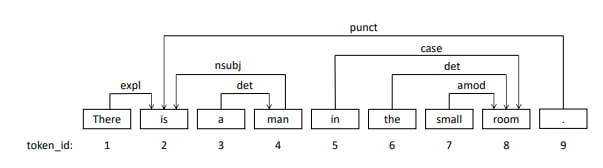
\includegraphics[width = \textwidth]{chapter/chapter3/figure3.7.jpg}
    \caption{An example of a parsed sentence.}
    \label{fig:placeholder37}
\end{figure}

\section{Calculating the Weights in the Bag-of-Words
Model}

When it is clear which features will be used to describe the processed document,
it is necessary to quantify them. Every feature in each document is then given
a weight that somehow represents its importance. The value is generally calculated based on the number of occurrences of words in every document and in the
entire collection. The weight \( w_{ij} \) of every term i in document j is given by three
components \cite{ref236}:

\begin{itemize}
    \item \textit{a local weight l\( w_{ij} \)} representing the frequency in every single document,

    \item \textit{a global weight} g\( w_{i} \) reflecting the discriminative ability of the term, based
on the distribution of the term in the entire document collection, and

    \item \textit{a normalization factor \( n_{j} \)} correcting the impact of different document
lengths.
\end{itemize}

The weight \( w_{ij} \) is then calculated according to the following formula:

\[
w_{ij} = \frac{l w_{ij} * g w_i}{n_j}
\tag{3.4}
\]

The local weight is the only mandatory weight which needs to be determined.
The other components do not have to be used at all.

\subsection{Local Weights}

A local weight quantifies the importance of a term in a \textit{single document}, not
considering the other documents. It is therefore based on the frequency of the
occurrence of the term in the specific document. The higher the frequency, the
higher is the weight.

In some situations, it is only important whether a word is present or absent in
a document. The weight is therefore \textit{binary}, also known as \textit{term presence}. Value
0 means that a documents does not contain a term, value 1 says that the word is
there, irrespective of its frequency. It is considered to be a baseline to measure
the usefulness of a term \cite{ref252}.

The most straightforward method of \textit{local term weighting} is to simply use
the \textit{term frequencies} as weights. If a term is not in a document, the value of the
weight is 0; if it is there once, the value is 1; for a double occurrence, the value
is 2, and so on. Thus, when a term appears ten times in a document, it is twice
as important as a term appearing five times and ten times more important than a
term that is present only once.


Such a direct proportionality, however, does not accurately represent the reality in some situations. When \textit{document A} contains a certain word five times and the other \textit{document B} only once, \textit{document A} is definitely more relevant, for example, in an information retrieval task. But is it really five times more important? Not necessarily. Consider another situation. When retrieving documents using a \textit{query} consisting of three words (\(q=\{w_1,w_2,w_3\}\)), a \textit{document A} containing word \(w_1\) four times and words \(w_2\) and \(w_3\) zero times (the sum of weights of the words shared by the document and the query will be 4) will be more relevant than a \textit{document B} containing all words once (the sum of weights will be 3). Intuitively, we would expect that \textit{document B} should be more relevant because it contains more query terms~\cite{ref252}.

To decrease the impact of high occurrences of a term, a few weights were developed. Buckley, Allan, and Salton~\cite{ref41} and Dumais~\cite{ref77} proposed an application of the \textit{logarithm} so that the weight grows less than linearly. The \textit{augmented normalized term frequency} puts the values to a certain range, \(k\) to 1 (often, \(k = 0.5\))~\cite{ref235}. A single occurrence of a given term has some minimal weight, and any additional occurrence increases it up to 1. This can be understood as a form of normalization based on the maximal frequency of a term in a document.

For a detailed description of the mentioned and some other local weights, see
Table 3.3. A graph demonstrating how the values of local weights grow, together
with increasing term frequencies is contained in Figure 3.8.

\subsection{Global Weights}

The goal of global weights is to decrease the importance of terms that are too
common. Some English words, like the, appear in almost every English text.
Thus, this word has no impact on, for example, the categorization of a newspaper article under the sports or politics category. Neither does it contribute much
to determining a similarity between two documents. Its influence on the results
of information retrieval are also negligible. We, therefore, want to decrease the
weight of such words and give a higher weight to words that do not appear so
often so they have a higher discriminative power. This means that we need to
consider the distribution of words in the entire document collection.

The Inverse Document Frequency (IDF) \cite{ref227} is probably the most popular
global weight. It is the logarithm of the inverse probability that a term appears in
a random document. When a term is contained in every document, the probability
of its appearance is 1 and the logarithm equals to 0. This means that this term has
no impact on any subsequent calculation. Inverse document frequency, together
with term frequency, is probably the most popular weighting scheme known as
term frequency-inverse document frequency or simply tf-idf .

A probabilistic version of the IDF is the logarithm of the odds that a
term appears in a random document \cite{ref49}. Entropy is the most sophisticated
\cite{ref187} information-theoretic measure \cite{ref77} taking values between 0 and 1. Some

\begin{table}[H]
\centering
\caption{Calculating the local weight for term $i$ in document $j$ where $f_{ij}$ is the frequency of term $i$ in document $j$, 
$a_j$ is $\mathrm{average}(f_j)$, $x_j$ is $\mathrm{max}(f_j)$, $k$ is a user specified constant between 0 and 1, 
$l_{\mathrm{avg}}$ is the average document length, $l_j$ is the length of document $j$.}
\renewcommand{\arraystretch}{1.3}
\begin{tabular}{l|l}
\hline
\textbf{Weight name} & \textbf{Calculation} \\
\hline
Binary (Term Presence) & 
$\begin{cases}
l w_{ij} = 0 & \text{if } f_{ij} = 0 \\
l w_{ij} = 1 & \text{if } f_{ij} > 0
\end{cases}$ \\

\hline
Term Frequency (TF) & $l w_{ij} = f_{ij}$ \\

\hline
Squared TF & $l w_{ij} = f_{ij}^2$ \\

\hline
Thresholded TF & 
$\begin{cases}
l w_{ij} = 0 & \text{if } f_{ij} = 0 \\
l w_{ij} = 1 & \text{if } f_{ij} = 1 \\
l w_{ij} = 2 & \text{if } f_{ij} \ge 2
\end{cases}$ \\

\hline
Logarithm &
$\begin{cases}
l w_{ij} = 0 & \text{if } f_{ij} = 0 \\
l w_{ij} = \log(f_{ij} + 1) & \text{if } f_{ij} > 0
\end{cases}$ \\

\hline
Alternate Logarithm &
$\begin{cases}
l w_{ij} = 0 & \text{if } f_{ij} = 0 \\
l w_{ij} = 1 + \log f_{ij} & \text{if } f_{ij} > 0
\end{cases}$ \\

\hline
Normalized Logarithm &
$\begin{cases}
l w_{ij} = 0 & \text{if } f_{ij} = 0 \\
l w_{ij} = \frac{1 + \log f_{ij}}{1 + \log a_j} & \text{if } f_{ij} > 0
\end{cases}$ \\

\hline
Augmented Normalized TF &
$\begin{cases}
l w_{ij} = 0 & \text{if } f_{ij} = 0 \\
l w_{ij} = k + (1 - k) \left( \frac{f_{ij}}{x_j} \right) & \text{if } f_{ij} > 0
\end{cases}$ \\

\hline
Changed-coefficient Average TF &
$\begin{cases}
l w_{ij} = 0 & \text{if } f_{ij} = 0 \\
l w_{ij} = k + (1 - k) \frac{f_{ij}}{a_j} & \text{if } f_{ij} > 0
\end{cases}$ \\

\hline
Square Root &
$\begin{cases}
l w_{ij} = 0 & \text{if } f_{ij} = 0 \\
l w_{ij} = \sqrt{f_{ij}} - 0.5 + 1 & \text{if } f_{ij} > 0
\end{cases}$ \\

\hline
Augmented Logarithm &
$\begin{cases}
l w_{ij} = 0 & \text{if } f_{ij} = 0 \\
l w_{ij} = k + (1 - k) \log(f_{ij} + 1) & \text{if } f_{ij} > 0
\end{cases}$ \\

\hline
Augmented Average TF &
$\begin{cases}
l w_{ij} = 0 & \text{if } f_{ij} = 0 \\
l w_{ij} = k + (1 - k) \frac{f_{ij}}{a_j} & \text{if } f_{ij} > 0
\end{cases}$ \\

\hline
DFR-like Normalization &
$l w_{ij} = f_{ij} \times \frac{l_{\mathrm{avg}}}{l_j}$ \\

\hline
Okapi's TF Factor &
$l w_{ij} = \frac{f_{ij}}{2 + f_{ij}}$ \\
\hline
\end{tabular}
\end{table}

other measures, together with necessary calculation formulae, can be found in
Table 3.4.

\subsection{Normalization Factor}
The basic idea behind document length normalization is based on two aspects:

\begin{itemize}
    \item \textit{Longer documents contain more distinct terms:} This significantly influences the similarity between documents because more matches exist in
individual dimensions in the vector space. This is very obvious in an information retrieval task where there is a higher chance that a query will be
matched against longer documents rather than against shorter documents.
\end{itemize}

\begin{figure}[!ht]
    \centering
    % \includegraphics[width=0.5\linewidth]{}
    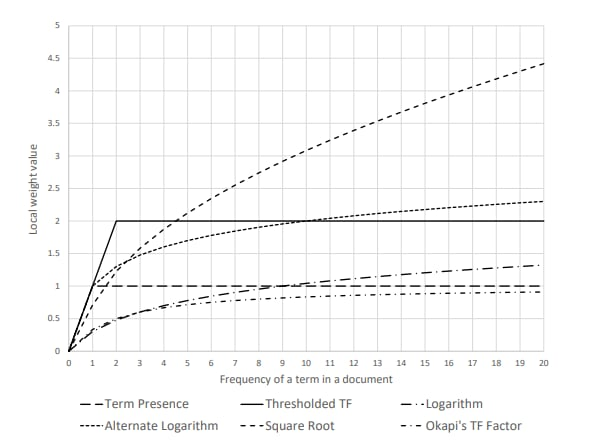
\includegraphics[width = \textwidth]{chapter/chapter3/figure3.8.jpg}
    \caption{Dependence between the number of occurrences of a term in a document and the
values of selected local weights.}
    \label{fig:placeholder38}
\end{figure}

\begin{itemize}
    \item \textit{Term frequencies in longer documents are higher}: In the case of two documents, one consisting of 50 words where Prague appears five times and
the other of 1,000,000 words containing Prague six times, the first one
is definitely related to the Czech Republic more than the second, even
though it has a lower frequency of the word Prague. When looking at the
frequency relatively, the word Prague represents one fifth of all words
in the first document whereas in the second document, it is a negligible
fraction.
\end{itemize}

In order to calculate the normalization factor, weights of the vector are combined to a single number. These weights are the local weights multiplied by
global weights (when used).

The most commonly used normalization technique is \textbf{cosine normalization}.
It simply transforms a vector to a unit vector (a vector of length 1) by dividing
it by its length (calculated as $\sqrt{w_1^2 + w_2^2 + \cdots + w_m^2}$).
This simultaneously addresses both reasons for document length normalization -- high frequencies as well as 

\begin{table}[!ht]
\centering
\caption{Calculating global weights for term $i$ where $N$ is the number of documents in the collection, $n_i$ is the number of documents containing term $i$ (document frequency), $f_{ij}$ is the frequency of term $i$ in document $j$, $F_i$ is the global frequency of term $i$, and $l_j$ is the length of document $j$.}
\begin{tabular}{l|l}
\hline
\textbf{Weight name} & \textbf{Calculation} \\ \hline
None & $gw_i = 1$ \\ \hline
Inverse Document Frequency (IDF) & $gw_i = \log \frac{N}{n_i}$ \\ \hline
Squared IDF & $gw_i = \log^2 \frac{N}{n_i}$ \\ \hline
Probabilistic IDF & $gw_i = \log \frac{N - n_i}{n_i}$ \\ \hline
Global frequency IDF & $gw_i = \frac{F_i}{n_i}$ \\ \hline
Entropy & $gw_i = 1 + \sum_{j=1}^{N}\frac{\frac{f_{ij}}{F_i} \log \frac{f_{ij}}{F_i}}{\log N}$ \\ \hline
Incremented global frequency IDF & $gw_i = \frac{F_i}{n_i} + 1$ \\ \hline
Log-global frequency IDF & $gw_i = \log \left( \frac{F_i}{n_i} + 1 \right)$ \\ \hline
Square root global frequency IDF & $gw_i = \sqrt{\frac{F_i}{n_i}} - 0.9$ \\ \hline
Inverse total term frequency & $gw_i = \log \frac{\sum_{j=1}^{N} l_j}{F_i}$ \\ \hline
\end{tabular}
\end{table}

\begin{table}[!ht]
\centering
\caption{Normalization of weights in document $j$, where $gw_i$ is the value of the global weight of term $i$, $lw_{ij}$ is the value of the global weight of term $i$ in document $j$, $m$ is the number of terms in document $j$, and $f_{ij}$ is the frequency of term $i$ in document $j$.}

\begin{tabular}{l|l}
\hline
\textbf{Weight name} & \textbf{Calculation} \\ \hline
None & $n_j = 1$ \\ \hline
Cosine & $n_j = \sqrt{\sum_{i=1}^{m} (gw_i * lw_{ij})^2}$ \\ \hline
Sum of weights & $n_j = \sum_{i=1}^{m} gw_i * lw_{ij}$ \\ \hline
Max weight & $n_j = \max gw_i * lw_{ij}$ \\ \hline
Max TF & $n_j = 0.5 + 0.5 * \frac{gw_i * lw_{ij}}{\max gw_i * lw_{ij}}$ \\ \hline
Square root & $f_{ij} = \sqrt{gw_i * lw_{ij}}$ \\ \hline
Logarithm & $f_{ij} = \log gw_i * lw_{ij}$ \\ \hline
Fourth normalization & $n_j = \sqrt[4]{\sum_{i=1}^{m} (gw_i * lw_{ij})^4}$ \\ \hline
\end{tabular}
\end{table}

\hspace{-1.5em}a larger number of terms (non-zero elements) in a document; as a result, the
normalization factor has a higher value \cite{ref252}. This kind of normalization also has
another positive effect. In order to calculate the cosine similarity of two vectors (see section 12.3.1) only the dot product of these vectors needs to be calculated
\cite{ref185}.

Other methods include dividing every vector component by the maximal
value in the vector which shrinks the components’ values to the range 0 to 1
\cite{ref216} or scaling to the range 0.5 to 1 by adding one half of the ratio between a
vector component and the maximal value to 0.5 \cite{ref141}.

\section{Common Formats for Storing Structured Data}

After some of the preprocessing steps mentioned above have been carried out
and the values of the document-term matrix components have been calculated,
the data is ready for further processing by machine learning algorithms. The data
is now in an internal form in the operational memory of the given software package performing the conversion to a structured representation. When the software
has the necessary capabilities, data mining algorithms can be applied to the data.
When a different data mining software is used (for example, when it implements
a specific algorithm with much higher speed of computation), the data usually
needs to be stored to a file with the specific structure required by that software
and loaded there. This section describes a few common formats for storing structured data which are often used in machine learning.

\subsection{Attibute-Relation File Format(ARFF)}

The \textit{Attribute-Relation File Format} (ARFF) is a format developed by the Machine Learning Project at the Department of Computer Science of The University of Waikato for use with their Weka machine learning software \cite{ref280}. A file
having this format consists of a header and data sections.

The header contains the name of a relation and a list of attributes, together
with their data types. A relation name as well as an attribute name is a string
(double quoted when containing spaces). The data type can be one of the four
following types:

\begin{itemize}
    \item numeric – integer or real numbers
    \item <nominal-specification> – a list of possible values is enumerated between a pair of curly brackets, comma separated (values containing
spaces need to be quoted)
    \item string – text values
    \item date [<date-format>] – date and time values, optionally with a specification of how to parse them (\textit{yyyy-MM-dd’T’HH:mm:ss} by default)
\end{itemize}

The data section contains one instance on every row. An instance is represented by a comma separated list of values in the order given in the header section. Strings and nominal values containing spaces must be quoted; dates are
always quoted. Missing values are represented by a single question mark.

An example of an ARFF file containing e-mails to be classified as spam and
ham can be found in Figure 3.9. In this example, the e-mail texts are in their
original textual form. When the raw text data is transformed to a structured representation, more attributes will appear. This is visible in Figure 3.10.

From Figure 3.10 is obvious that, even in the case of this simple example,
most of the values in the vectors are zeros (they are sparse). When a data set
contains a number of texts, the vectors are usually very large and the problem
is intensified. This also means that the ARFF files tend to occupy a large space
on the disks because they store many unnecessary zero values. To overcome this
problem, it is possible to store only non-zero values. It is, however, necessary
to add an index to each such value. The indices start from 0 and the values are
stored in space separated pairs <index> <value>. Every instance is enclosed in
a pair of curly brackets. An example of a sparse ARFF file is in Figure 3.11.

Both ARFF and sparse ARFF files can be stored in a XML-based format
known as eXtensible attribute-Relation File Format (XRFF). The format is able
to include some additional properties of a data set like class attribute specification, attribute weights, and instance weights to its description. In a sparse XRFF
file, an index for each value needs to be specified as an attribute of the <value>
element. Unlike in the sparse ARFF format, the indices begin with 1. Examples
of XRFF files for the e-mails dataset can be found in Figures 3.12 and 3.13.

\subsection{Comma-Separated Values(CSV)}

The \textit{comma-separated values} format is a very simple format for structured data
interchange.

\begin{verbatim}
@relation e-mails
@attribute text string
@attribute class {spam, ham}
@data
‘Want buy cheap V*I*A*G*R*A?’,spam
‘The meeting will take place on Monday.’,ham
‘A new version of our product will be launched next week.’,ham
‘Need help with transferring funds from Africa’,spam
\end{verbatim}

\begin{figure}[!ht]
    \centering
    % \includegraphics[width=0.5\linewidth]{}
    \caption{An example of an ARFF file containing e-mails to be classified as either \textit{spam or
ham}.}
    \label{fig:placeholder39}
\end{figure}

\begin{verbatim}
@relation "e-mails structured"

@attribute Africa numeric
@attribute Need numeric
@attribute V*I*A*G*R*A numeric
@attribute Want numeric
@attribute buy numeric
@attribute cheap numeric
@attribute from numeric
@attribute funds numeric
@attribute help numeric
@attribute transferring numeric
@attribute with numeric
@attribute A numeric
@attribute Monday numeric
@attribute The numeric
@attribute be numeric
@attribute launched numeric
@attribute meeting numeric
@attribute new numeric
@attribute next numeric
@attribute of numeric
@attribute on numeric
@attribute our numeric
@attribute place numeric
@attribute product numeric
@attribute take numeric
@attribute version numeric
@attribute week numeric
@attribute will numeric
@attribute class {spam,ham}

@data
0,0,1,1,1,1,0,0,0,0,0,0,0,0,0,0,0,0,0,0,0,0,0,0,0,0,0,0,spam
0,0,0,0,0,0,0,0,0,0,0,0,1,1,0,0,1,0,0,0,1,0,1,0,1,0,0,1,ham
0,0,0,0,0,0,0,0,0,0,0,1,0,0,1,1,0,1,1,1,0,1,0,1,0,1,1,1,ham
1,1,0,0,0,0,1,1,1,1,1,0,0,0,0,0,0,0,0,0,0,0,0,0,0,0,0,0,spam
\end{verbatim}

\begin{figure}[H]
    \centering
    % \includegraphics[width=0.5\linewidth]{}
    \caption{An example of an ARFF file containing e-mails to be classified as \textit{spam} or \textit{ham}.
The data is already transformed to a structured representation (bag-of-words model) when no
special preprocessing techniques have been applied.}
    \label{fig:placeholder310}
\end{figure}

Each line in a CSV file contains one instance. The attributes of each instance
are separated by commas and they are always in the same order. When a comma
(which normally separates values) or a line break (which generally denotes the
end of a record) is contained in a data field, the value should be enclosed between

\begin{verbatim}
@relation "e-mails sparse"

@attribute Africa numeric
@attribute Need numeric
...
@attribute class {spam,ham}

@data
{2 1,3 1,4 1,5 1,28 spam}
{12 1,13 1,16 1,20 1,22 1,24 1,27 1,28 ham}
{11 1,14 1,15 1,17 1,18 1,19 1,21 1,23 1,25 1,26 1,27 1,28 ham}
{0 1,1 1,6 1,7 1,8 1,9 1,10 1,28 spam}
\end{verbatim}

\begin{figure}[H]
    \centering
    % \includegraphics[width=0.5\linewidth]{}
    \caption{An example of an ARFF file containing e-mails to be classified as spam or ham.
The data is already transformed to a structured representation (bag-of-words model) when no
special preprocessing techniques have been applied. Instead of the sparse vectors that contain
many zeros, dense vectors are used.
}
    \label{fig:placeholder311}
\end{figure}

\hspace{-1.5em}a pair of double quotes. In such a situation, every double-quote appearing in a
field must be escaped by preceding it with another double quote.

Optionally, a CSV file can include a header containing attribute names on the
first line. The format of a header is the same as for the rest of the file.

Although the format is standardized \cite{ref248}, many variations based on the
above mentioned principles exist. For example, a tabulator can be used to separate the values instead of commas, or a line end different from CRLF can be
considered.

An example of a CSV file containing structured representation of e-mails is
in Figure 3.14.

\subsection{C5 format}

C5 (a UNIX version) and See5 (a Windows version) are very efficient data mining tools, enabling the construction of decision trees or rules and using them for
classification and prediction \cite{ref220}.

The data to be processed by the C5 package is divided into several files. They
share the same name called a filestem. An extension then defines what aspect of
the data is stored in the file named \textit{<filestem>}.\textit{<extension>}.

A file with an extension names defines the attributes and a file with an extension data contains the values of the instances to be processed. These two files
are required. The other three optional file types contain a data set for testing (extension test), instances to be classified (extension cases), and information about
misclassification costs (extension costs).

\begin{verbatim}
<dataset name="e-mails structured">
    <header>
        <attributes>
            <attribute name="Africa" type="numeric" />
            <attribute name="Need" type="numeric" />
            <attribute name="V*I*A*G*R*A" type="numeric" />
            ...
            <attribute name="class" type="nominal">
                <labels>
                    <label>spam</label>
                    <label>ham</label>
                </labels>
            </attribute>
        </attributes>
    </header>

    <body>
        <instances>
            <instance>
                <value>0</value>
                <value>0</value>
                <value>1</value>
                ...
                <value>spam</value>
            </instance>

            <instance>
                <value>0</value>
                <value>0</value>
                <value>0</value>
                ...
                <value>ham</value>
            </instance>

            ...
        </instances>
    </body>
</dataset>
\end{verbatim}

\begin{figure}[H]
    \centering
    % \includegraphics[width=0.5\linewidth]{}
    \caption{An example of an XRFF file containing e-mails to be classified as spam or ham.
The data is already transformed to a structured representation (bag-of-words model) when no
special preprocessing techniques have been applied. Instead of the sparse vectors that contain
many zeros, dense vectors are used.
}
    \label{fig:placeholder312}
\end{figure}

The program generates files with extensions tree or rules containing the generated decision tree or rules.

In the \textit{\texttt{names}} file, specification of a class is the first information. A class can
be defined in three different ways:

\begin{itemize}
    \item a comma separated list of class labels, e.g., \texttt{spam}, \texttt{ham}.
\end{itemize}

\begin{verbatim}
<dataset name="e-mails structured">
    <header>
        ...
    </header>

    <body>
        <instances>
            <instance type="sparse">
                <value index="3">1</value>
                ...
                <value index="5">spam</value>
            </instance>

            <instance type="sparse">
                <value index="1">1</value>
                <value index="5">ham</value>
            </instance>
        </instances>
    </body>
</dataset>
\end{verbatim}

\begin{figure}[H]
    \centering
    % \includegraphics[width=0.5\linewidth]{}
    \caption{An example of a XRFF file containing e-mails to be classified as spam or ham.
The data is already transformed to a structured representation (bag-of-words model) when no
special preprocessing techniques have been applied. Instead of the sparse vectors that contain
many zeros, dense vectors are used. The header section is the same as in case of the dense
XRFF example.}
    \label{fig:placeholder313}
\end{figure}

\begin{verbatim}
Africa,Need,V*I*A*G*R*A,...,week,will,class
0,0,1,1,1,1,0,0,0,0,0,0,0,0,0,0,0,0,0,0,0,0,0,0,0,0,0,0,spam
0,0,0,0,0,0,0,0,0,0,0,0,1,1,0,0,1,0,0,0,1,0,1,0,1,0,0,1,ham
0,0,0,0,0,0,0,0,0,0,0,1,0,0,1,1,0,1,1,1,0,1,0,1,0,1,1,1,ham
1,1,0,0,0,0,1,1,1,1,1,0,0,0,0,0,0,0,0,0,0,0,0,0,0,0,0,0,spam
\end{verbatim}

\begin{figure}[H]
    \centering
    % \includegraphics[width=0.5\linewidth]{}
    \caption{An example of a CSV file containing e-mails to be classified as spam or ham.
The data is already transformed to a structured representation (bag-of-words model) when no
special preprocessing techniques have been applied.}
    \label{fig:placeholder314}
\end{figure}


\begin{itemize}
    \item the name of a discrete attribute to be used as a class
    \item The name of a continuous attribute together with thresholds separating all
possible values to a countable number of intervals, e.g., \textit{age: 21, 50},
defines three classes ($age \leq 21$, $21 < age \leq 50$, and $50 \leq age$).
\end{itemize}

A list of all attribute names, together with their data types, follows.
A data type is separated by a colon from an attribute name. A few data
types are available: continuous for numeric values, date for dates (in
the form YYYY/MM/DD or YYYY-MM-DD), time for times (in the form
HH:MM:SS with values between 00:00:00 and 23:59:59), timestamp combining date and time (in the form YYYY/MM/DD HH:MM:SS or YYYY-MM-DD
HH:MM:SS), a comma-separated list of names enumerating the allowable values (e.g., \texttt{risk}: \texttt{low, medium, high}), \texttt{discrete} N for discrete, unordered
values that are assembled from the data itself, ignore for attributes to be ignored, and label for naming and referring the instances (labels are ignored
during processing). Attributes can be also defined by formulae, e.g., \texttt{Difference
:= A - B}.

At the end, optional information that explicitly specifies what attributes
should be processed can be included. This either lists the processed attributes
as \texttt{attributes included: a1, a3, a5}. or contains the attributes that will
not be used, like \texttt{attributes excluded: a2, a4}.

A data file contains the values of training instances. Each instance contains a
comma separated list of values for all explicitly-defined attributes. If the classes
are listed in the first line of the names file, the last value on each line is a class label. A question mark is used to denote a missing or unknown value, \texttt{N/A} denotes
a value that is not applicable. The values of the attributes that are calculated from
other attributes are naturally not included.

The test and cases files have the same format as the data file. In the cases
file, the class vales can be unknown.

An example of names and data file can be found in Figure 3.15.

\begin{center}
    file \textit{emails.names:}
\end{center}

\begin{verbatim}
spam, ham.
Africa : continuous.
Need : continuous.
VIAGRA : continuous.
...
week : continuous.
will : continuous.
\end{verbatim}

\begin{center}
    file \textit{emails.data}
\end{center}

\begin{verbatim}
0,0,1,1,1,1,0,0,0,0,0,0,0,0,0,0,0,0,0,0,0,0,0,0,0,0,0,0,spam
0,0,0,0,0,0,0,0,0,0,0,0,1,1,0,0,1,0,0,0,1,0,1,0,1,0,0,1,ham
0,0,0,0,0,0,0,0,0,0,0,1,0,0,1,1,0,1,1,1,0,1,0,1,0,1,1,1,ham
1,1,0,0,0,0,1,1,1,1,1,0,0,0,0,0,0,0,0,0,0,0,0,0,0,0,0,0,spam
\end{verbatim}

\begin{figure}[H]
    \centering
    % \includegraphics[width=0.5\linewidth]{}
    \caption{An example of files suitable for the C5 package. They describe e-mails to be
classified as spam or ham. The data is already transformed to a structured representation (bagof-words model) when no special preprocessing techniques have been applied.}
    \label{fig:placeholder315}
\end{figure}

\subsection{Matrix Files for CLUTO}

CLUTO is a software package for clustering low- and high-dimensional datasets
and for analyzing the characteristics of the various clusters. It contains many
clustering algorithms, similarity/distance functions, clustering criterion functions, agglomerative merging schemes, methods for effectively summarizing the
clusters, and visualization capabilities \cite{ref141}.

A matrix file (*.mat) contains a dense matrix, sparse matrix, or dense/sparse
similarity graph representing the data to be clustered.

The first row of a dense matrix contains the number of rows and columns of
the matrix. The remaining rows contain one instance on each row. The rows have
a form of space separated floating point values, including non-zero values. A
sparse matrix contains the number of rows, columns, and non-zero values of the
matrix on the first row. The remaining rows contain one instance on each row.
The rows have a form of space separated pairs of indexes and corresponding
non-zero values (which do not need to be ordered). The indexes begin with 1.

A dense graph format contains the number of vertices of the graph on the first
row. The remaining rows contain an adjacency matrix, which is a matrix n × n
where n is the number of vertices. An element on position i and j is a floating
point value representing the similarity of the ith and the jth vertex of the graph.
A sparse graph format contains the numbers of vertices and edges of the graph
on the first row. The remaining rows contain an adjacency matrix in the form of
index-value pairs (the indexes begin with 1).

Additionally, CLUTO accepts an rlabel file containig labels for the rows of
the data matrix, clabel file with labels for the columns of the data matrix, and
rclass file containing class labels for the rows of the data matrix for an external
cluster evaluation.

\subsection{SVMlight Format}

The format was developed by Thorsten Joachims to describe the data to be processed by his famous SMV\textsuperscript{\textit{light}} package that implements the support vector machine (SVM) algorithm \cite{ref135}.

Every line in a file represents one training example. The first value is a target
and can be one of the following values: $+1$, $-1$, $0$, or a floating point number.
The classes are normally labeled as $-1$ and $+1$. A class label of $0$ indicates that
this example should be classified using transduction. The target can also contain
a real number which is used in the regression mode.

A list of feature-value pairs follows. A feature is described by its number,
where the first feature has number 1. A value is a floating point number. The
target value and each of the feature-value pairs, which must be ordered by increasing feature numbers, are separated by a space character. Features with zero
values do not have to be included, which is common for sparse formats.

\begin{center}
file \textit{emails.mat} (sparse format):
\end{center}

\begin{verbatim}
4 28 29
3 1 4 1 5 1 6 1
13 1 14 1 17 1 21 1 23 1 25 1 28 1
12 1 15 1 16 1 18 1 19 1 20 1 22 1 24 1 26 1 27 1 28 1
1 1 2 1 7 1 8 1 9 1 10 1 11 1
\end{verbatim}

\begin{center}
file \textit{emails.rlabelfile}:
\end{center}

\begin{verbatim}
spam
ham
ham
spam
\end{verbatim}

\begin{center}
file \textit{emails.clabel:}
\end{center}

\begin{verbatim}
Africa
Need
VIAGRA
...
week
will
\end{verbatim}

\begin{figure}[H]
    \centering
    % \includegraphics[width=0.5\linewidth]{}
    \caption{An example of files suitable for the CLUTO package. They describe e-mails to
be classified as spam or ham. The data is already transformed to a structured representation
(bag-of-words model) when no special preprocessing techniques have been applied.}
    \label{fig:placeholder316}
\end{figure}

Every row can be followed by a string starting with \#. It is then used as
additional information to a user defined kernel.

An example of a SVMlight file can be found in Figure 3.17.

\begin{verbatim}
1 3:1 4:1 5:1 6:1
-1 13:1 14:1 17:1 21:1 23:1 25:1 28:1
-1 12:1 15:1 16:1 18:1 19:1 20:1 22:1 24:1 26:1 27:1 28:1
1 1:1 2:1 7:1 8:1 9:1 10:1 11:1
\end{verbatim}

\begin{figure}[H]
    \centering
    % \includegraphics[width=0.5\linewidth]{}
    \caption{An example of a file in the SVMlight format describing e-mails to be classified
as spam or ham. The data is already transformed to a structured representation (bag-of-words
model) when no special preprocessing techniques have been applied.}
    \label{fig:placeholder317}
\end{figure}

\subsection{Reading Data in R}

There are a few packages which provide functions implementing the reading of
data from common formats.

The \texttt{read.arff()} function from package RWeka reads data from AttributeRelation File Format (ARFF) files. The only input parameter is a character string with the name of the file or a connection. The function returns a data frame
containing the data.

To read data in a tabular format, including CSV files, the function
\texttt{read.table()} can be used. The function reads a file in table format and creates
a data frame from it. The lines correspond to individual instances and fields on
each line correspond to attributes of the instances. Using input parameters, a user
can specify whether the file contains a header, identify the field separator character,
specify how strings are quoted, which character is used for decimal points,
what is the maximum number of rows to read, or how many lines of the data
to skip. The functions \texttt{read.csv()} and \texttt{read.csv2()}, intended for reading the
content of CSV files, are identical to \texttt{read.table()} but have different default
values for their parameters.

Using the function \texttt{C45Loader()} from package RWeka, data in the C4.5 format (which is identical to the C5 format described above) can be read.

Package skmeans provides function \texttt{readCM()} that reads a sparse matrix in
the CLUTO format and returns a triplet matrix (values are represented by triplets
– row index, column index, value) defined by the indexR packages!slamslam
package.

To save data in a format of R, the function \texttt{save()} can be used. It accepts
a list of whatever objects are written to a file (with an extension \texttt{.RData}) with
the name given as the parameter, \texttt{file}. These objects can be read later and the
structures in the memory recreated using function \texttt{load()} where the parameter
is the file name with stored objects.

\section{A Complex Example}

Like in almost every major statistical computing product, R also offers text mining capabilities. A well-known text mining framework, \texttt{tm} is an open source
package providing the basic infrastructure necessary to organize, transform, and
analyze textual data \cite{ref86}.

A document collection can be represented by an object of class \texttt{VCorpus}
(Volatile Corpus, a default implementation, documents are stored in the volatile
memory) or \texttt{PCorpus} (Permanent Corpus, where the documents are stored
outside an R program). The first parameter of the methods creating a corpus
(\texttt{VCorpus()} or \texttt{PCorpus()}) is a \texttt{Source} class object which specifies the source
of the data.

A number of methods, each handling data in different formats, may be used
to create the corpus. The complete list of available sources is returned by the
\texttt{getSources()} function. It includes, for example:

\begin{itemize}
    \item \texttt{VectorSource()} – each element of a vector is interpreted as a document.

    \item \texttt{DataFrameSource()} – the corpus is created for a data frame where the
first column is names \texttt{doc\_id} (a unique string identifier) and the second
column is text (a UTF-8 encoded string).

    \item \texttt{DirSource()} – each file in a directory is treated as a document.

    \item \texttt{URISource()} – the data from a specified URI is used to form a document.
\end{itemize}

The data from a specified source is read by a function known as a reader.
The behaviour of the reader is influenced by the parameter \texttt{readerControl}.
This is a list with components \texttt{reader}, specifying a particular reader to be
used, and \texttt{language}, defining the language of the documents. The readers (their
complete list is returned by the function \texttt{getReaders()}) include, for example,
\texttt{readDataframe} (reads data from a data frame), \texttt{readDOC} (reads data from a Microsoft Word document), \texttt{readPDF} (reads data from a Portable Document Format
document), \texttt{readPlain} (reads texts from a list with a content component), or
\texttt{readXML} (reads an XML document). In addition to an object containing the data,
all functions also accept additional information suitable for a specific data source
(for example, the name of a PDF extraction engine for reading PDF documents).
A language (\texttt{en} by default) is passed as an IETF language tag.

The documents in a corpus can be modified using the \texttt{tm\_map()} function.
This function applies another function known as a transformation to all documents in a corpus. The list of transformations, which can be retrieved by the
\texttt{getTransformations()} function, includes:

\begin{itemize}
    \item \texttt{removeNumbers()} – removes numbers; a logical parameter, \texttt{ucp}, specifies whether to use Unicode character properties for determining digit
characters.

    \item \texttt{removePunctuation()} – removes punctuation. With the parameter
\texttt{preserve\_intra\_word\_contractions} – a user specifies whether intraword contractions should be kept; the 
\texttt{preserve\_intra\_word\_dashes} parameter controls the removal of intra-word dashes. 
The parameter \texttt{ucp} determines the punctuation characters. They include 
$$! " \# \$ \% \& ' ( ) * + , - . / : ; < = > ? @ [ ] ^ ` \{ | \} ~$$ when 
\texttt{FALSE} (by default), or the Unicode punctuation characters when \texttt{TRUE}.

    \item \texttt{removeWords()} – returns a document without the words specified as the
second parameter (or a parameter named \texttt{words}). This function is often
used to remove stop words. The list can be returned by the \texttt{stopwords()}
function with a parameter specifying the language.

    \item \texttt{stemDocument()} – performs stemming using the Porter’s stemming algorithm. An optional parameter, \texttt{language}, can be used to choose
a proper Snowball stemmer.

    \item \texttt{stripWhitespace()} – replaces multiple whitespaces with a single
space in a document.
\end{itemize}

Custom transformations can be created with the \texttt{content\_transformer()}
function. This function accepts as a parameter another function which modifies
the content of an object with implemented content getter (\texttt{content}) and setter
(\texttt{content<-}) functions. An existing function as well as a function defined by a
programmer can be used, as demonstrated below:


\begin{verbatim}
# an existing function
c <- tm_map(c, content_transformer(tolower))

# a defined function replacing all e-mail addresses
# with "--email--"
email.replace <- content_transformer(
        function (x) gsub("([\\w.]+)@([\\w.]+\\.[a-z]+)",
                          "--email--",
                          x,
                          perl=TRUE)
        )
c <- tm_map(c, content_transformer(email.replace))
\end{verbatim}

The function \texttt{tm\_filter()} enables the selection of only the documents
which meet certain criteria. It returns a corpus containing documents where a
function passed as the second parameter returns \texttt{TRUE}. The function \texttt{tm\_index()}
works on the same principle but returns only a logical value for each document.

To save a corpus on a disk, the function \texttt{writeCorpus()} can be used. It takes
a corpus as an input and writes the content (applies \texttt{as.character()} to each
document) to files in a given location. Filenames are generated from document
IDs or from character strings passed as an optional parameter.

To create a document-term matrix (documents are in rows) or term-document matrix (terms are in rows), the functions \texttt{DocumentTermMatrix()}
and \texttt{TermDocumentMatrix()} can be used. Both functions implement sparse
matrices. The \texttt{as.matrix()} function can be used to display a full matrix. A
sample is displayed by the function \texttt{inspect()}.

To control the process of calculating the values (weights of the terms) in
the matrices, a named list, \textit{control}, with options is supplied. Local options are
evaluated for each document and global options are evaluated once for the entire
matrix.

The local options include:

\begin{itemize}
    \item \texttt{tokenize} – a function tokenizing a document into single tokens. The
function can be one of predefined functions or a user-defined one.
    \item \texttt{tolower} – a logical value indicating whether characters should be translated to lower case or a custom function converting characters to lower
case.
    \item \texttt{language} – the language (preferably as an IETF language tag) to be used
for the removal of stop words and stemming.
    \item \texttt{removePunctuation} – a logical value indicating whether punctuation
characters should be removed, a function performing punctuation removal, or a list of arguments for \texttt{removePunctuation()}.
    \item \texttt{removeNumbers} – a logical value indicating whether numbers should be
removed or a function implementing number removal.
    \item \texttt{stopwords} – a Boolean value indicating stop word removal using default
language-specific stop words lists, a character vector holding custom stop
words, or a custom function for stop words removal.
    \item \texttt{stemming} – a Boolean value indicating whether tokens should be
stemmed or a custom stemming function.
    \item \texttt{stemming} – a Boolean value indicating whether tokens should be
stemmed or a custom stemming function.
    \item \texttt{dictionary} – a character vector containing acceptable terms; other
terms in the documents will be ignored.
    \item \texttt{bounds} – a list with a tag \texttt{local} containing an integer vector of length
two. The first value specifies the minimal number of occurrences of a
term in a document, the second value defines the maximal number of
occurrences of the term in a document.
    \item \texttt{wordLengths} – an integer vector of length two. The values define the
minimal and maximal lengths of a term.
\end{itemize}

Global options include:

\begin{itemize}
    \item \texttt{bound} – a list with tag global which contains an integer vector with two
elements. The elements are the lower and upper bounds for the document
frequency of a term. Terms that are out of the bounds are eliminated.
\end{itemize}

\begin{verbatim}
# eliminating terms that appear less than twice
tdm <- TermDocumentMatrix(
       c,
       control=list(bounds=list(global=c(2, Inf)))
      )
\end{verbatim}

\begin{itemize}
    \item \texttt{weighting} – a weighting function. The \texttt{tm} package provides \texttt{weightTf}
(term frequency, a default option), \texttt{weightTfIdf} (term frequency – inverse document frequency), \texttt{weightBin} (binary weighting, term presence/absence), and \texttt{weightSMART} options. The \texttt{weightSMART} option defines weights in SMART notation. Three characters in a string passed as
a parameter specify the local and global components and a normalization
factor. The local weights include term frequency (\texttt{n}), logarithm (\texttt{l}), augmented normalized term frequency (\texttt{a}), term presence (\texttt{b}), and normalized logarithm also known as log average (\texttt{L}). The global options include
no weighting (\texttt{n}), inverse document frequency (\texttt{t}), and probabilistic IDF (\texttt{p}). The vectors can be normalized using the cosine normalization (\texttt{c}),
pivoted normalization (\texttt{u}), byte size (\texttt{b}), or do not have to be normalized (\texttt{n}).
\end{itemize}

A useful function which reduces the sparsity of a matrix representing the
documents is \texttt{removeSparseTerms()}. It removes terms that have a higher percentage of empty (zero) values in a document term matrix than the parameter (a
value between 0 and 1).

There are a few functions which provide some basic information about the
content of a term-document matrix or document-term matrix, which is a parameter of these functions. These functions include \texttt{Docs()} (returns document IDs),
\texttt{Terms()} (returns a list of terms), \texttt{nDocs()} (returns the number of documents),
and \texttt{nTerms()} (returns the number of terms).

The function \texttt{findMostFreqTerms()} calculates and returns the frequencies of words in every document or group of documents (given by the \texttt{INDEX}
object) ordering the frequency in descending order. A maximum number of
words (parameter \texttt{n}) can be given. The documents are in the form of a term-document matrix, document-term matrix, or a vector of frequencies returned by
\texttt{termFreq()} (which calculates term frequencies for a single document).

The function \texttt{plot()} visualizes correlations between the terms of a termdocument matrix (it requires the Rgraphviz library) in the form of a graph where
the vertices (terms) are connected by edges (associations). Terms to be plotted
(20 terms, randomly chosen by default) and correlation threshold are some of the
possible parameters.

To visualize Zipf’s law and Heaps’ law based on the values contained in a
document-term matrix or term-document matrix with unweighted term frequencies, tm provides the functions \texttt{Zipf\_plot()} and \texttt{Heaps\_plot()}. A user can
specify the type of plot to be drawn and further graphical parameters to be used
for plotting.

An example of using the \texttt{tm} package for analyzing a corpus and for preparing
a document term matrix follows.

\begin{verbatim}
> d <- c("The Vegas Golden Knights ice hockey team
+ achieved the milestone of most home wins.",
+ "Germany won 1-0 over Argentina in the FIFA Wold
+ Cup finals.",
+ "Someone has won tonight’s USD 10 million jackpot
+ in the National Lottery.",
+ "A man has won a USD 10 million jackpot on
+ a Las Vegas slot machine.")

> # creating a corpus from a character vector
> c <- VCorpus(VectorSource(d))

> # looking at some basic information about the corpus
> c
<<VCorpus>>
Metadata: corpus specific: 0, document level (indexed): 0
Content: documents: 4

> # looking at the text of the second document
> c[[2]]$content # same as as.character(c[[2]])
[1] "Germany won 1-0 over Argentina in the FIFA Wold
Cup finals."

> # finding only documents that contain the word "Vegas"
> c2 <- tm_filter(c,
+ FUN=function(x)
+ any(grep("Vegas", content(x))))
> lapply(c2, as.character)
$‘1‘
[1] "The Vegas Golden Knights ice hockey team achieved the
milestone of most home wins."
$‘4‘
[1] "A man has won a USD 10 million jackpot on a Las
Vegas slot machine."

> # finding indices of documents that contain the word "Vegas"
> tm_index(c, FUN=function(x)
+ any(grep("Vegas", content(x))))
[1] TRUE FALSE FALSE TRUE

> # writing the documents from the filtered corpus to a directory "filtered_corpus"
> writeCorpus(c2, path="filtered_corpus")

> # removing numbers from the documents
> c <- tm_map(c, removeNumbers)

> # looking at the text of all documents
> lapply(c, as.character)
$‘1‘
[1] "The Vegas Golden Knights ice hockey team achieved
the milestone of most home wins."
$‘2‘
[1] "Germany won - over Argentina in the FIFA Wold Cup
finals."
$‘3‘
[1] "Someone has won tonights USD million jackpot in
the National Lottery."
$‘4‘
[1] "A man has won a USD million jackpot on a Las
Vegas slot machine."

> # removing punctuation
> c <- tm_map(c, function(x)
+ removePunctuation(
+ x,
+ preserve_intra_word_contractions=FALSE))

> # performing stemming
> c <- tm_map(c, stemDocument)

> # looking at the text of all documents after transformations
> lapply(c, as.character)
$‘1‘
[1] "The Vega Golden Knight ice hockey team achiev the
mileston of most home win"
$‘2‘
[1] "Germani won over Argentina in the FIFA Wold Cup final"
$‘3‘
[1] "Someon has won tonight USD million jackpot in the
Nation Lotteri"
$‘4‘
[1] "A man has won a USD million jackpot on a Las Vega
slot machin"

> # generating a document-term matrix
> dtm <- DocumentTermMatrix(c)

> # display detailed information on the document-term matrix
> inspect(dtm)
<<DocumentTermMatrix (documents: 4, terms: 32)>>
Non-/sparse entries: 41/87
Sparsity : 68%
Maximal term length: 9
Weighting : term frequency (tf)
Sample :
Terms
Docs achiev argentina cup has jackpot million the usd
1 1 0 0 0 0 0 2 0
2 0 1 1 0 0 0 1 0
3 0 0 0 1 1 1 1 1
4 0 0 0 1 1 1 0 1
Terms
Docs vega won
1 1 0
2 0 1
3 0 1
4 1 1

> # displaying the document-term matrix as a matrix
> as.matrix(dtm)
Docs achiev argentina cup fifa final ...
1 1 0 0 0 0 ...
2 0 1 1 1 1 ...
3 0 0 0 0 0 ...
4 0 0 0 0 0 ...

> # looking at some properties of the document-term matrix
> Docs(dtm)
[1] "1" "2" "3" "4"

> nDocs(dtm)
[1] 4

> Terms(dtm)
[1] "achiev" "argentina" "cup" "fifa"
[5] "final" "germani" "golden" "has"
[9] "hockey" "home" "ice" "jackpot"
[13] "knight" "las" "lotteri" "machin"
[17] "man" "mileston" "million" "most"
[21] "nation" "over" "slot" "someon"
[25] "team" "the" "tonight" "usd"
[29] "vega" "win" "wold" "won"

> nTerms(dtm)
[1] 32

> # looking at 5 most frequent terms in the entire collection
> findMostFreqTerms(dtm, INDEX=rep(1, times=nDocs(dtm)),n=5)
$‘1‘
the won has jackpot million
4 3 2 2 2

> # removing columns that have more than a half of zero elements
> dtm2 <- removeSparseTerms(dtm, 0.51)
> as.matrix(dtm2)
Terms
Docs has jackpot million the usd vega won
1 0 0 0 2 0 1 0
2 0 0 0 1 0 0 1
3 1 1 1 1 1 0 1
4 1 1 1 0 1 1 1

> # storing data to a CSV file to be used later
> m <- as.matrix(dtm2)
> write.csv(m, file="data.csv")
\end{verbatim}

As an alternative to the package tm, a natural language processing toolkit
udpipe can be used. The package provides tokenization, part of speech tagging,
lemmatization, and dependency parsing capabilities. It also enables training annotation models, converting texts to a document-term matrix, and some basic
operations with the matrix.

The function \texttt{udpipe()} analyzes text and returns a data frame where one row
corresponds to one token in the data. The fields contain a document identifier (\texttt{doc id}), a paragraph identifier unique within each document (\texttt{paragraph id}),
a sentence identifier unique within each document (\texttt{sentence id}), the text of
the sentence (\texttt{sentence}), integer indices indicating the beginning and end of
the token in the original text (\texttt{start}, \texttt{end}), a row identifier unique
within the document (\texttt{term id}), a token index starting at 1 for each sentence
(\texttt{token id}), the token (\texttt{token}), the lemma of the token (\texttt{lemma}),
the universal and treebank-specific part of speech tags of the token (\texttt{upos}, \texttt{xpos}),
the morphological features of the token separated by \texttt{|} (\texttt{feats}), indicating
what token id in the sentence the token is related to (\texttt{head token id}) and
what type of relation it is (\texttt{dep rel}), enhanced dependency graph (\texttt{deps}),
and information about spaces in a token used to reconstruct the original text (\texttt{misc}).

The function \texttt{document\_term\_frequencies(d)} calculates the number of
times a term occurs per document. The input is a data frame, data table, or character vector (it needs to be split first according to the submitted optional parameter split). The output is a data table with columns \texttt{doc\_id}, \texttt{term}, and \texttt{freq}
indicating how many times a term occurred in each document.

A data table returned by the function \texttt{document\_term\_frequencies()} 
can be passed to \texttt{document\_term\_frequencies\_statistics()}. 
This function adds term frequency normalized by the number of terms in a document, 
inverse document frequency, and Okapi BM25 statistics to the output.

The output from the \texttt{document\_term\_frequencies(d)} function
can be converted to a document-term matrix using the function
\texttt{document\_term\_matrix()}. The matrix is a sparse object of class \texttt{dgCMatrix}
with the documents in the rows and the terms in the columns. Optionally, a vocabulary can be supplied using the \texttt{vocabulary} parameter. In such a case, only
terms which are in the vocabulary will be in the matrix.

Two sparse matrices can be joined using \texttt{dtm\_cbind()} or \texttt{dtm\_rbind()} (by
columns or by rows).

The functions \texttt{dtm\_colsums()} and \texttt{dtm\_rowsums(dtm)} return column sums
and row sums for a document term matrix.

Using the function \texttt{dtm\_remove\_lowfreq()}, terms occurring with low frequency and documents with no terms are removed from a document-term matrix. The minimal frequency is given by the \texttt{minfreq} parameter. An optional
parameter, \texttt{maxterms}, indicates the maximum number of terms to be kept in the
matrix. Similarly, the function \texttt{dtm\_remove\_tfidf()} removes terms with low
tf-idf frequencies.

To eliminate specific terms, the function \texttt{dtm\_remove\_terms()} can be used.
The terms are passed as the terms parameter.

\begin{verbatim}
> library(udpipe)
> udpipe("Machine learning is great. Learn it!",
+ object="english")
doc_id paragraph_id sentence_id
1 doc1 1 1 Machine learning is great.
2 doc1 1 1 Machine learning is great.
3 doc1 1 1 Machine learning is great.
4 doc1 1 1 Machine learning is great.
5 doc1 1 1 Machine learning is great.
6 doc1 1 2 Learn it!
7 doc1 1 2 Learn it!
8 doc1 1 2 Learn it!
start end term_id token_id token lemma upos xpos
1 1 7 1 1 Machine machine NOUN NN
2 9 16 2 2 learning learning NOUN NN
3 18 19 3 3 is be AUX VBZ
4 21 25 4 4 great great ADJ JJ
5 26 26 5 5 . . PUNCT .
6 28 32 6 1 Learn Learn VERB VB
7 34 35 7 2 it it PRON PRP
8 36 36 8 3 ! ! PUNCT .
feats
1 Number=Sing
2 Number=Sing
3 Mood=Ind|Number=Sing|Person=3|Tense=Pres|VerbForm=Fin
4 Degree=Pos
5 <NA>
6 Mood=Imp|VerbForm=Fin
7 Case=Acc|Gender=Neut|Number=Sing|Person=3|PronType=Prs
8 <NA>
head_token_id dep_rel deps misc
1 2 compound <NA> <NA>
2 4 nsubj <NA> <NA>
3 4 cop <NA> <NA>
4 0 root <NA> SpaceAfter=No
5 4 punct <NA> <NA>
6 0 root <NA> <NA>
7 1 obj <NA> SpaceAfter=No
8 1 punct <NA> SpacesAfter=\\n

> d <- c("Good product!",
+ "Bad product.",
+ "Not very good product.",
+ "Not bad.",
+ "Very very good.")
> d <- tolower(d)
> df <- document_term_frequencies(d)
> df
doc_id term freq
1: doc1 good 1
2: doc1 product 1
3: doc2 bad 1
4: doc2 product 1
5: doc3 not 1
6: doc3 very 1
7: doc3 good 1
8: doc3 product 1
9: doc4 not 1
10: doc4 bad 1
11: doc5 very 2
12: doc5 good 1

> document_term_frequencies_statistics(df)
> df
doc_id term freq tf idf tf_idf
1: doc1 good 1 0.5000000 0.5108256 0.2554128
2: doc1 product 1 0.5000000 0.5108256 0.2554128
3: doc2 bad 1 0.5000000 0.9162907 0.4581454
4: doc2 product 1 0.5000000 0.5108256 0.2554128
5: doc3 not 1 0.2500000 0.9162907 0.2290727
6: doc3 very 1 0.2500000 0.9162907 0.2290727
7: doc3 good 1 0.2500000 0.5108256 0.1277064
8: doc3 product 1 0.2500000 0.5108256 0.1277064
9: doc4 not 1 0.5000000 0.9162907 0.4581454
10: doc4 bad 1 0.5000000 0.9162907 0.4581454
11: doc5 very 2 0.6666667 0.9162907 0.6108605
12: doc5 good 1 0.3333333 0.5108256 0.1702752
tf_bm25 bm25
1: 1.1042471 0.5640777
2: 1.1042471 0.5640777
3: 1.1042471 1.0118114
4: 1.1042471 0.5640777
5: 0.8194842 0.7508858
6: 0.8194842 0.7508858
7: 0.8194842 0.4186135
8: 0.8194842 0.4186135
9: 1.1042471 1.0118114
10: 1.1042471 1.0118114
11: 1.3179724 1.2076458
12: 0.9407895 0.4805794

> df <- document_term_frequencies(d)
> dtm <- document_term_matrix(df)
> dtm
5 x 5 sparse Matrix of class "dgCMatrix"
bad good not product very
doc1 . 1 . 1 .
doc2 1 . . 1 .
doc3 . 1 1 1 1
doc4 1 . 1 . .
doc5 . 1 . . 2

> dtm_colsums(dtm)
bad good not product very
2 3 2 3 3

> dtm_rowsums(dtm)
doc1 doc2 doc3 doc4 doc5
2 2 4 2 3

> dtm_remove_terms(dtm, terms = c("product"))
5 x 4 sparse Matrix of class "dgCMatrix"
bad good not very
doc1 . 1 . .
doc2 1 . . .
doc3 . 1 1 1
doc4 1 . 1 .
doc5 . 1 . 2

> as.matrix(dtm)
bad good not product very
doc1 0 1 0 1 0
doc2 1 0 0 1 0
doc3 0 1 1 1 1
doc4 1 0 1 0 0
doc5 0 1 0 0 2
\end{verbatim}




